\documentclass[../master]{subfiles}

%\graphicspath{{../eps/}}

\begin{document}

\chapter{シミュレーションによるトラックの再現}
\label{chap::simulation}
\section{\texorpdfstring{$\alpha$}{alpha}線源を用いた測定}
\ref{sec::detection_gas_candidate}節で考えた各検出ガスについて,
シミュレーションの基準となるトラックを測定した.
また,それらのデータから各ガスにおけるドリフトスピード,ガスの電子増幅率,トラックの幅を測定した.
測定には${}^{241}{\rm Am}$の$\alpha$線源を用いた.
図\ref{fig::a_source_track}に$\alpha$線源のトラックの一例を示す.
図\ref{fig::a_source_track}では検出ガスに\isoButaneHydro を用いた.
\ref{sec::detection_gas_candidate}節では6種類の候補を考えたが,
ここからは単体のiso-$\rm C_{4}H_{10}$を除いた5種類について考えていく.
これはディフュージョン係数が大きくトラックが太くなると予測されることと,
圧力が\SI{15}{\hecto\pascal}と低く安定したTPC の動作が難しいと予測されるためである.
\begin{figure}
  \centering
  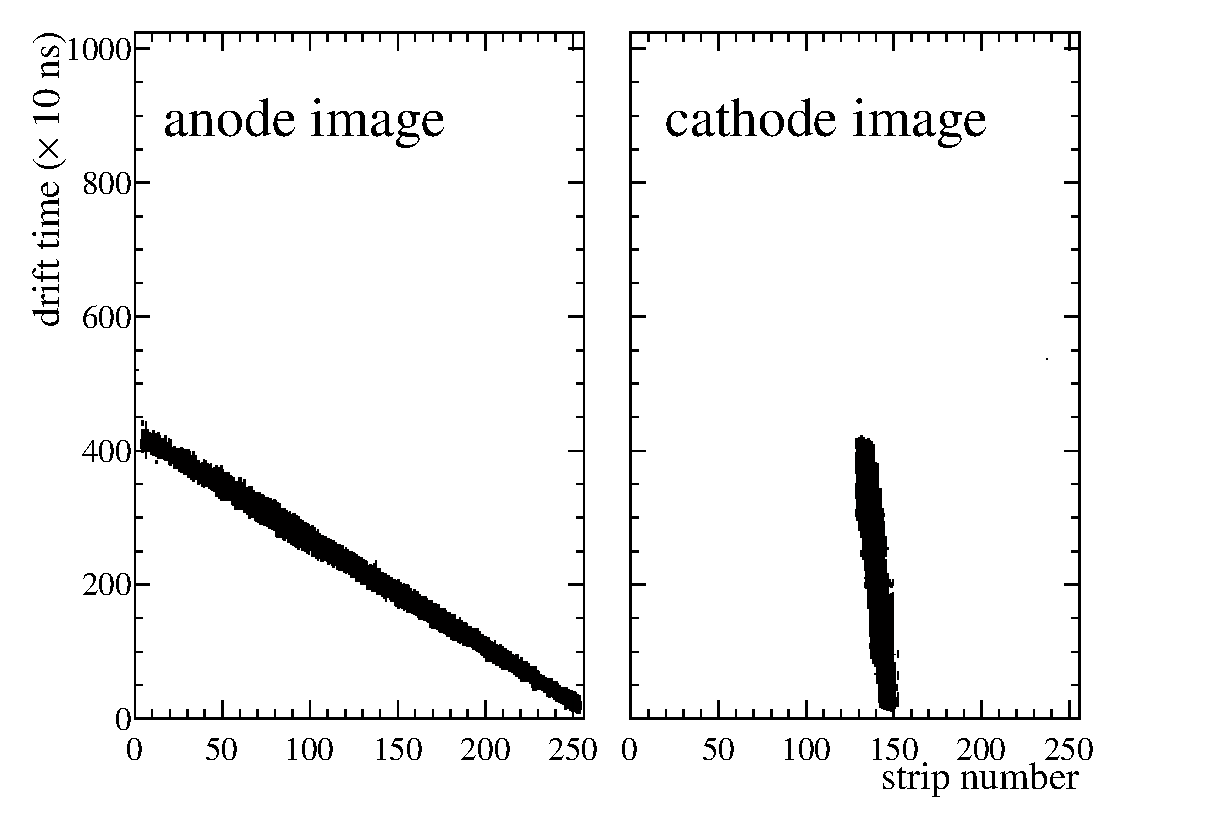
\includegraphics[clip, width=0.9\columnwidth]{0210_7.eps}
  \caption[$\alpha$線源で測定したトラックの一例.]
          {$\alpha$線源で測定したトラックの一例.
          検出ガスは\isoButaneHydro を用いた.}
  \label{fig::a_source_track}
\end{figure}

\subsection{ドリフトスピード}
電子のドリフトスピードを線源によって得られるトラックから求める.
測定には図\ref{pic::alpha_collimator}のような線源コリメータを用いる.
このコリメータはアクリルで作られており,1つの\ang{0}と4つの\ang{30}の穴が開いている.
このコリメータを用いることで$\alpha$線を\ang{0}と\ang{30}の方向に限定することができる.
\ang{30}方向の$\alpha$線は図\ref{fig::drift_v_image}の右のようにドリフト方向に$\Delta y$~\si{\milli\metre},
それと垂直な方向に$\Delta z$~\si{\milli\metre}移動するとき,
\begin{equation}
  \Delta y = \tan(\ang{30})\times\Delta z \label{eq::deltay_deltaz}
\end{equation}
となる.
MAIKo TPC で取得したトラックの横方向の変分を$\Delta strip$,縦方向の変分を$\Delta t$~\si{\nano\second},
ドリフトスピードを$v_{\text{drift}}$~\si{\milli\metre\per\nano\second}とすると,
\begin{align}
  \frac{\Delta z}{\SI{0.4}{\milli\metre}} & = \Delta strip \label{eq::deltaz}\\
  \frac{\Delta y}{v_{\text{drift}}} & = \Delta t \label{eq::deltay}
\end{align}
という関係にある.
式\eqref{eq::deltay_deltaz}, \eqref{eq::deltaz}, \eqref{eq::deltay} より
\begin{equation}
  v_{\text{drift}} = \frac{\tan(\ang{30})\times\Delta strip\times\SI{0.4}{\milli\metre}}{\Delta t}
\end{equation}
とドリフトスピードが求まる.
\begin{figure}
  \centering
  \begin{subfigure}{0.45\columnwidth}
    \centering
    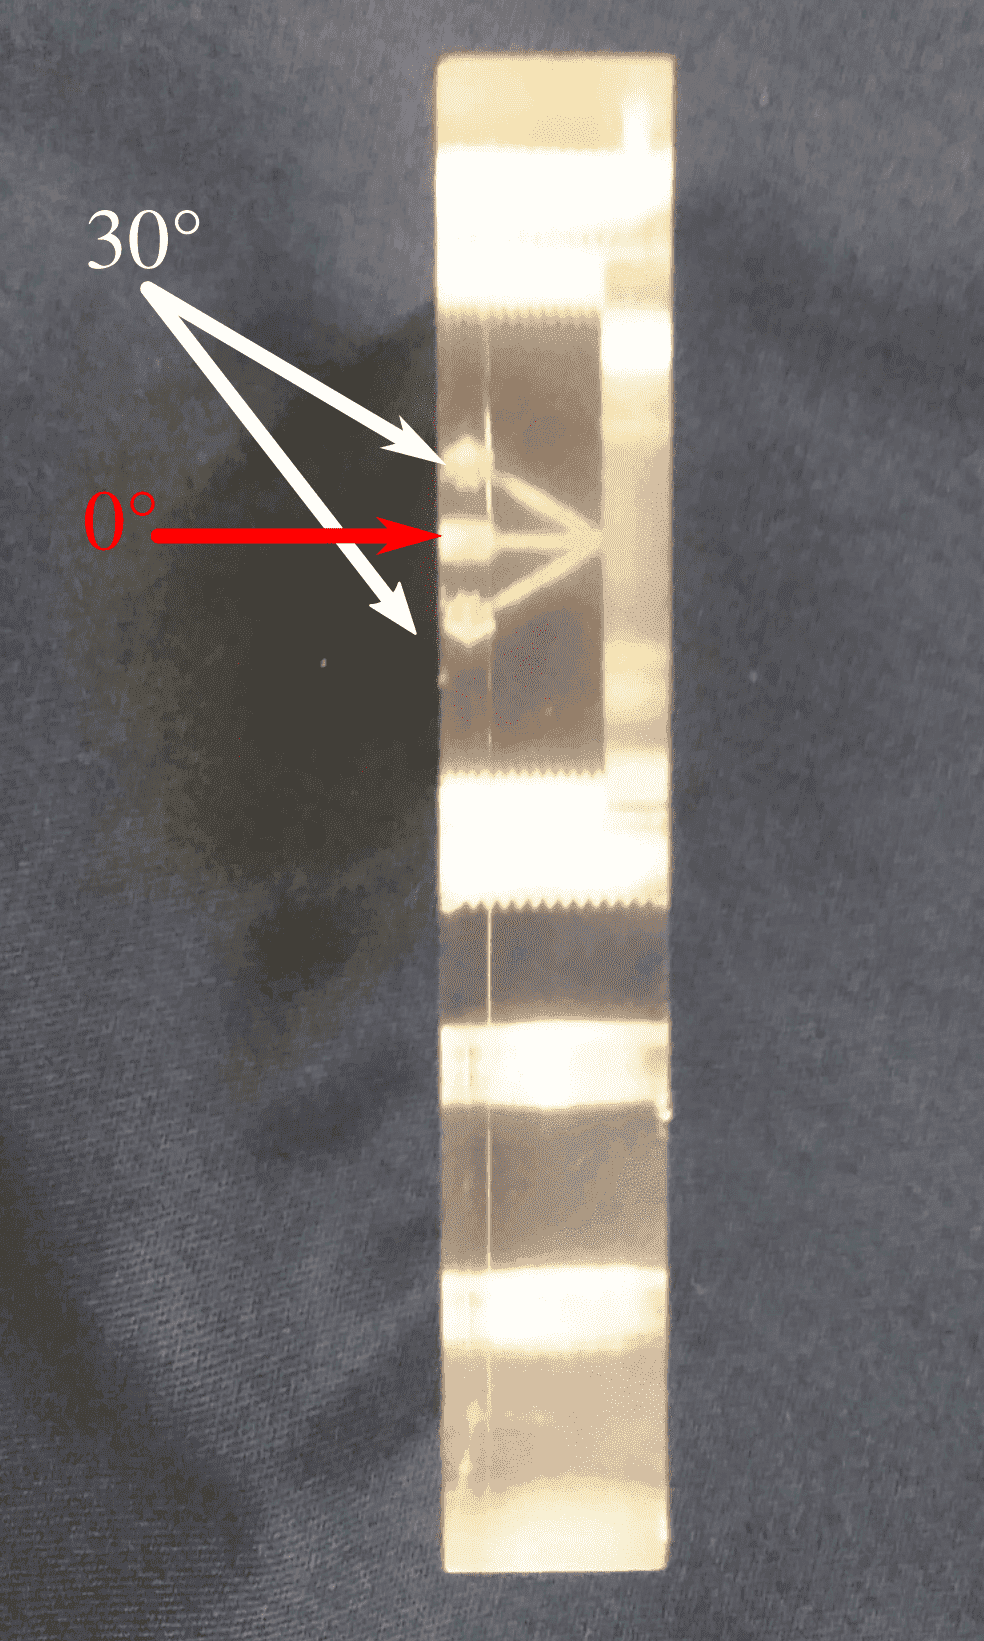
\includegraphics[clip, width=0.8\columnwidth]{image30580-min.png}
    \caption{側面.}
  \end{subfigure}
  \begin{subfigure}{0.45\columnwidth}
    \centering
    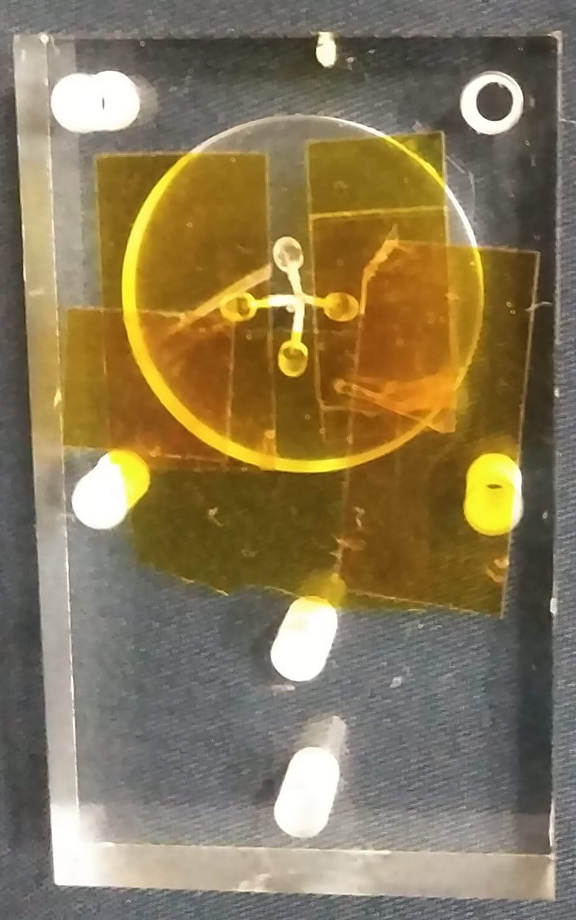
\includegraphics[clip, width=0.8\columnwidth]{IMG_20191225_183542_clip.jpg}
    \caption{正面.}
  \end{subfigure}
  \caption[線源コリメータ.]
          {線源コリメータ.中央に\ang{0},上下左右に\ang{30}の穴が開いている.
            \ang{0}の穴と1つの\ang{30}の穴を除いてカプトンテープで塞ぐことで,
            余計な$\alpha$線が出ないようにしている.
          }
          \label{pic::alpha_collimator}
\end{figure}
\begin{figure}
  \centering
  \begin{minipage}{0.45\columnwidth}
    \centering
    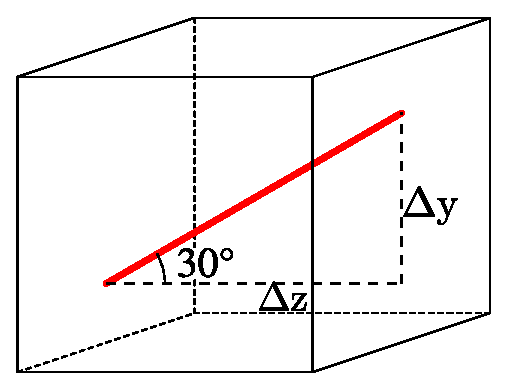
\includegraphics[clip, width=0.9\columnwidth]{drift_v_source.eps}
  \end{minipage}
  \begin{minipage}{0.45\columnwidth}
    \centering
    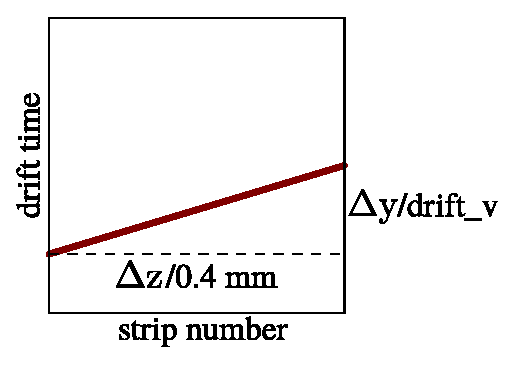
\includegraphics[clip, width=0.9\columnwidth]{drift_v_image.eps}
  \end{minipage}
  \caption[\ang{30}に方向を限定した$\alpha$線と取得される画像データのイメージ.]
          {\ang{30}に方向を限定した$\alpha$線 (左) と取得される画像データ (右) のイメージ.}
  \label{fig::drift_v_image}
\end{figure}

$\alpha$線源を用いて測定したドリフトスピードとMagboltz で求めた値を
表\ref{tab::drift_speed_compare}に示す.
$\alpha$線源を用いて測定したドリフトスピードと Magboltz を用いて計算したドリフトスピードがおおよそ一致していることが分かる.
ここで,Magboltz の計算値が\SI{0.014}{\milli\metre\per\nano\second}となっていないのは,
MAIKo TPC のオペレートを簡単にするために設定電圧を切りの良い値にしたためである.
\Methane は実測とMagboltz による計算値とがずれているが,検出ガスに含まれる水分の影響が考えられる.
\Methane のみ\SI{50}{\hecto\pascal} とその他のガスと比較して圧力が半分であるため,不純物の影響が大きく出ていると考えられる.
不純物のドリフトスピードへの影響は付録\ref{app::drift_speed_humid_dep}で述べる.
\begin{table}
  \centering
  \caption{実測したドリフトスピードとMagboltzで求めたドリフトスピードの比較.}
  \label{tab::drift_speed_compare}
  \begin{tabular}{cccc}
    \toprule
    gas & ドリフト電場 (\si{\volt\per\milli\metre}) & 実測 (\si{\milli\metre\per\nano\second})
    & Magboltz (\si{\milli\metre/\nano\second})\\
    \midrule
    \Methane & 0.429 & 0.0126 & 0.0145 \\
    \MethaneHydro & 4.32 & 0.0140 & 0.0140 \\
    \MethaneHerium & 1.89 & 0.0135 & 0.0140 \\
    \isoButaneHydro & 6.82 & 0.0137 & 0.0140 \\
    \isoButaneHerium & 3.29 & 0.0139 & 0.0141 \\
    \bottomrule
  \end{tabular}
\end{table}
%\begin{figure}
%  \centering
%  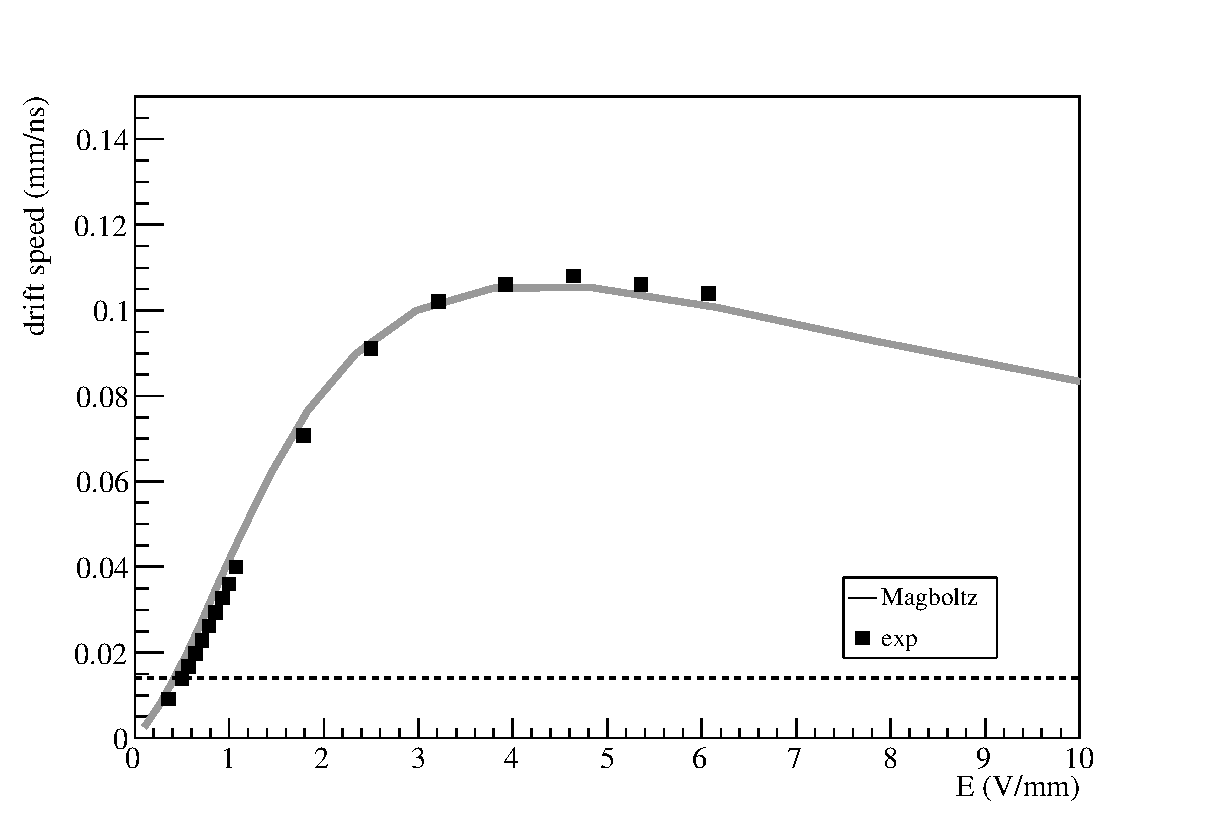
\includegraphics[clip, width=0.9\columnwidth]{drift_v_CH4.eps}
%  \caption[検出ガスに${\rm CH_{4}}$を用いたときのドリフトスピードの電場依存性.]
%          {検出ガスに${\rm CH_{4}}$を用いたときのドリフトスピードの電場依存性.
%            図中の点線は0.014 mm/ns を示す.}
%  \label{fig::drift_v_CH4}
%%  \includegraphics[clip, width=0.7\columnwidth]{drift_v_CH4_H2.eps}
%  \caption{}
%  \label{fig::drift_v_CH4_H2}
%%  \includegraphics[clip, width=0.7\columnwidth]{drift_v_CH4_He.eps}
%  \caption{}
%  \label{fig::drift_v_CH4_He}
%  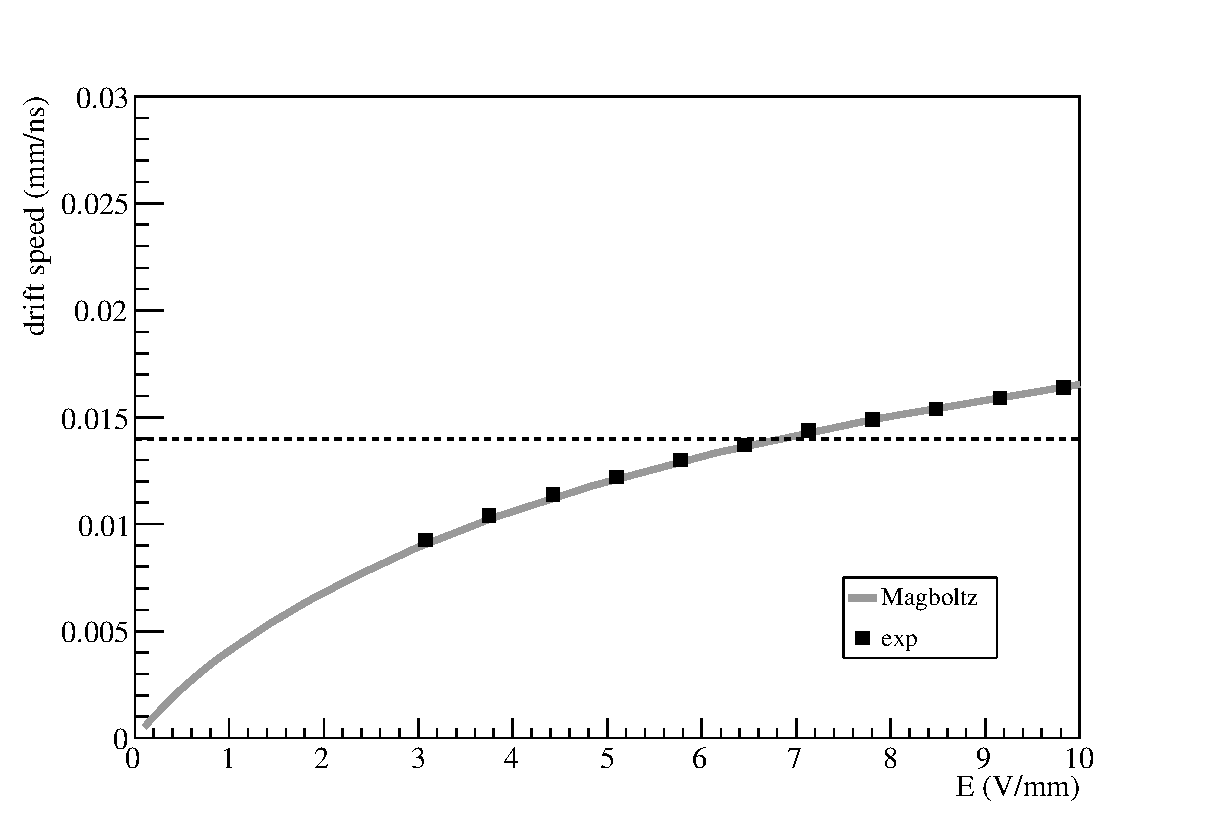
\includegraphics[clip, width=0.9\columnwidth]{drift_v_iC4H10_H2.eps}
%  \caption[検出ガスにiso-${\rm C_{4}H_{10}}$を用いたときのドリフトスピードの電場依存性.]
%          {検出ガスにiso-${\rm C_{4}H_{10}}$を用いたときのドリフトスピードの電場依存性.
%        p    図中の点線は0.014 mm/ns を示す.}
%  \label{fig::drift_v_iC4H10_H2}
%%  \includegraphics[clip, width=0.7\columnwidth]{drift_v_iC4H10_He.eps}
%  \caption{}
%  \label{fig::drift_v_iC4H10_He}
%\end{figure}

\subsection{電子増幅率}
各部の電圧に対する電子増幅率の依存性を測定した.
増幅率は荷電粒子が検出ガス中を通過した際に発生させた電子数 ($N_{\mathrm{e}}$) と
増幅後に$\mu$-PICによって収集された電子数 ($N'_{\mathrm{e}}$) から求めることができる.
$N_{\mathrm{e}}$は検出ガス中での荷電粒子のエネルギー損失と検出ガスのW値から求める.
$N'_{\mathrm{e}}$は$\mu$-PICで収集した電荷から求める.
詳しい計算方法について以下で述べる.

検出ガス中で荷電粒子がエネルギーを落とすと,W値あたり平均1個の電子を電離する.
そのため,荷電粒子のエネルギー損失をW値で割ることで$N_{\mathrm{e}}$が求まる.
各検出ガスのエネルギー損失とW値~\cite{energy_per_ion_pair,pdg}を表\ref{tab::energy_loss_and_W_val}に示す.
${}^{241}\mathrm{Am}$からは\SI{5.4}{\mega\electronvolt}の$\alpha$線が放出される.
測定に用いた$\alpha$線源は線量を大きくするために,多くの${}^{241}\mathrm{Am}$が線源に含まれている.
そのため,物質厚が大きくなっており,線源中でエネルギーを落としてしまう.
この線源から出ている$\alpha$粒子の持つエネルギーが平均\SI{4.2}{\mega\electronvolt}であることが他の測定によりわかっている.
本測定では\ang{0}方向の$\alpha$線を用いて測定した.
エネルギー損失は\SI{4.2}{\mega\electronvolt}の$\alpha$粒子が$\mu$-PIC 32 strip分の
距離 (\SI{12.8}{\milli\metre}) で落とすエネルギーを示している.
この距離で発生した電子が$\mu$-PIC の32 stripsで収集される.
\begin{table}
  \centering
  \caption[検出ガスのW値とエネルギー損失と$N_{\rm e}$.]
          {検出ガスのW値~\cite{energy_per_ion_pair,pdg}とエネルギー損失と$N_{\rm e}$.
          エネルギー損失は荷電粒子がガス中を\SI{12.8}{\milli\metre} 進んだ時のものである.}
  \label{tab::energy_loss_and_W_val}
  \begin{tabular}{cccc}
    \toprule
    gas & W値 (\si{\electronvolt}) & energy loss (\si{\kilo\electronvolt}) & $N_{\rm e}$\\
    \midrule
    \Methane         & 29.1 & 56.5 & 1.94$\times 10^{3}$ \\
    \MethaneHydro    & 34.2 & 53.4 & 1.56$\times 10^{3}$ \\
    \MethaneHerium   & 39.2 & 59.3 & 1.51$\times 10^{3}$ \\
%    iso-${\rm C_{4}H_{10}}$                 & 26.0 & 0.0552 & 2.12$\times 10^{3}$ \\
    \isoButaneHydro  & 35.4 & 62.0 & 1.75$\times 10^{3}$ \\
    \isoButaneHerium & 44.0 & 58.0 & 1.32$\times 10^{3}$ \\
    \bottomrule
  \end{tabular}
\end{table}

32 strips まとめた$\mu$-PICからの信号波形は図\ref{fig::FADC_waveform}のようなFADC 情報として取得している.
この信号波形を時間で積分することによって32 strips で収集した電荷量を計算することができる.
$\mu$-PICで取得した電気信号は読み出し回路内部で800倍に増幅され,
入力インピーダンス\SI{50}{\ohm}で電流値を電圧値に変換して取得している.
よって,式\eqref{eq::N'e}で$\mu$-PICで収集した電荷量を求めることができる.
\si{\elementarycharge}は電気素量である.
\begin{equation}
  N'_{\mathrm{e}} = \frac{\int V (t) dt}{ 50 \times 800 \times \si{\elementarycharge}}
  \label{eq::N'e}
\end{equation}
各検出ガスの増幅率と電子の収集効率を畳み込んだ値を表\ref{tab::multiplying_rate}に示す.
ここでは,GEMと$\mu$-PIC の両方による増幅率となっている.
\begin{table}
  \centering
  \caption{各検出ガスの電子増幅率.}
  \label{tab::multiplying_rate}
  \begin{tabular}{cc}
    \toprule
    gas & 増幅率 (倍) \\
    \midrule
    \Methane         & 700 \\
    \MethaneHydro    & 354 \\
    \MethaneHerium   & 322 \\
    \isoButaneHydro  & 272 \\
    \isoButaneHerium & 392 \\
    \bottomrule
  \end{tabular}
\end{table}

\subsection{幅}
本実験の目的である3$\alpha$に崩壊するイベントではトラックが太いと複数のトラックの区別が難しくなり,
トラックの抽出を正しくできなくなる.
そこで,\ang{0}の$\alpha$粒子によるトラックで幅を測定した.
図\ref{fig::track_width}に示すように,
トラックの幅にはanode strip 128~ch目のclock方向の幅を用いる.
このようにして決定したトラックの幅を表\ref{tab::track_width},図\ref{fig::diffusion_compare}に示す.
図\ref{fig::diffusion_compare}から分かるようにトラックの幅とディフュージョン係数には相関がある.
ディフュージョン係数,トラックの幅ともに\isoButaneHydro が最も小さいことが分かる.
\begin{figure}
  \centering
  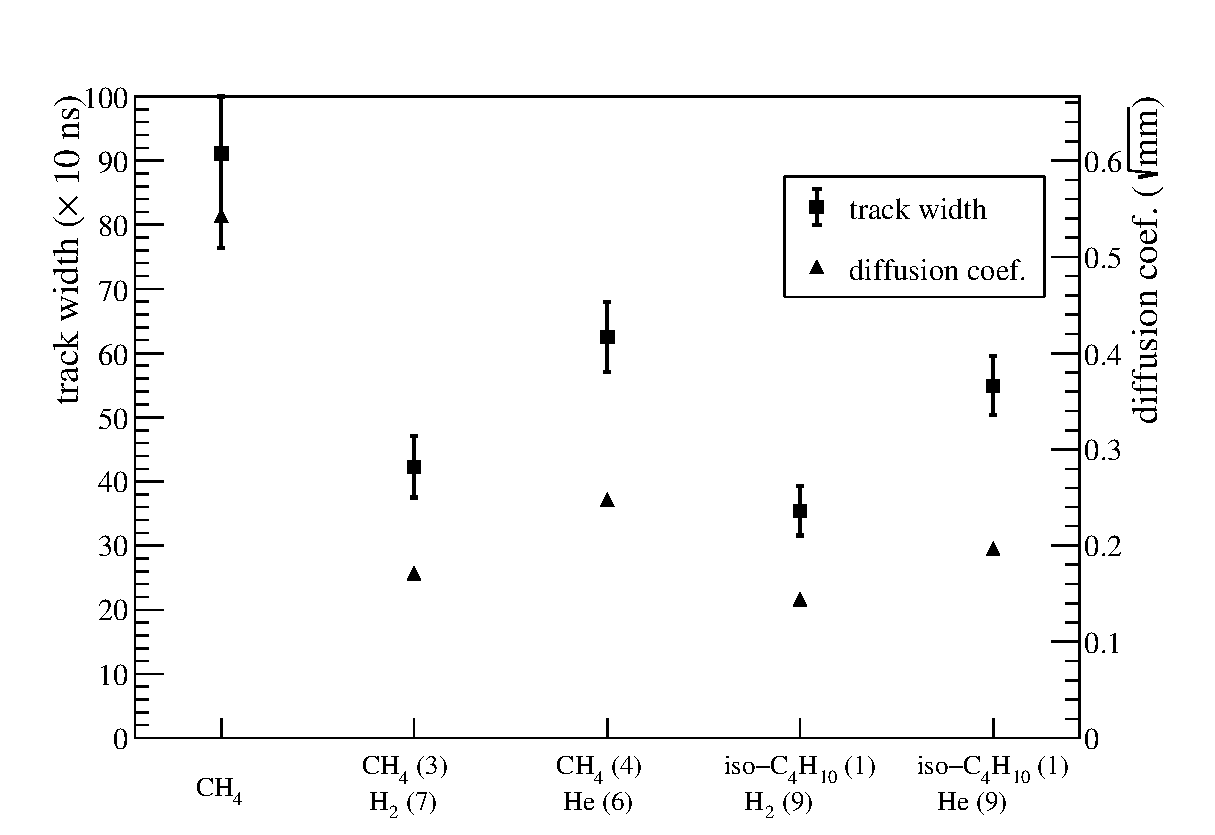
\includegraphics[clip, width=0.5\columnwidth]{track_width.eps}
  \caption{トラックの幅の決定方法のイメージ.
    トラックの幅は有感領域の中央であるanode strip 128~chのclock方向の幅を用いる.}
  \label{fig::track_width}
\end{figure}

%\begin{table}
%  \centering
%  \caption{各検出ガスでのトラックの幅.}
%  \label{tab::track_width}
%  \begin{tabular}{cc}
%    \toprule
%    gas & トラックの幅 ($\times \SI{10}{\nano\second}$)\\
%    \midrule
%    \Methane         & 91.1 \\
%    \MethaneHydro    & 42.3 \\
%    \MethaneHerium   & 62.5 \\
%    \isoButaneHydro  & 35.4 \\
%    \isoButaneHerium & 54.9 \\
%    \bottomrule
%  \end{tabular}
%\end{table}

\begin{figure}
  \centering
  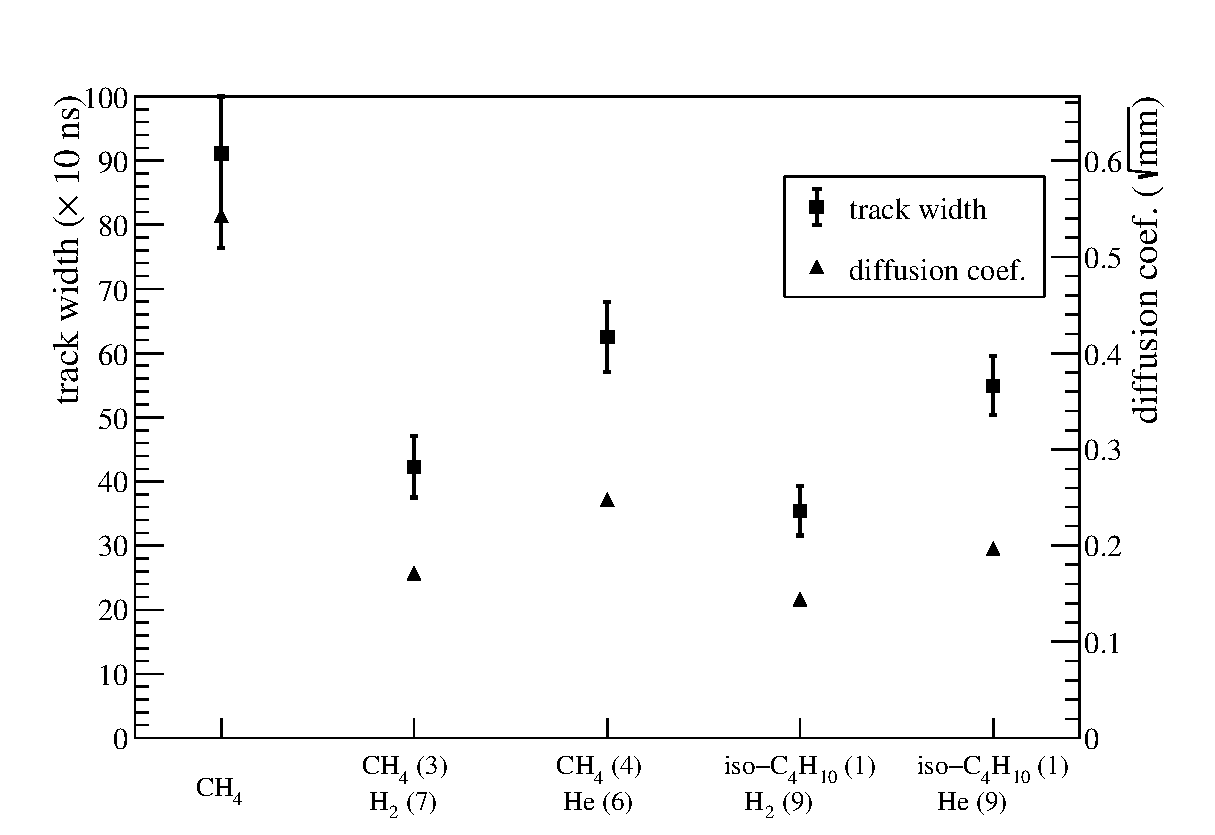
\includegraphics[clip, width=0.9\columnwidth]{diffusion_compare.eps}
  \caption{Magboltz で求めたディフージョン係数と実測によるトラックの幅.}
  \label{fig::diffusion_compare}
\end{figure}

\section{シミュレーションによる線源データの再現}
MAIKo TPC から得られるトラックをGarfield++~\cite{garfield++}と
Magboltz~\cite{magboltz},SRIM~\cite{SRIM}を用いたシミュレーションにより再現した.
シミュレーションでは,ドリフト電場,W値,電子増幅率,検出ガスの密度をfixed parameters,
TOTの閾値をfree parameterとした.
シミュレーションは以下のような手順%(図\ref{fig::simulation_flow})
で行った.
\begin{enumerate}
\item\label{sim::particle_generate}
  トラックを生成する荷電粒子のエネルギー,運動量を決定し,
  Garfield++のSrimTrack に登録する.
\item
  SrimTrack によりトラックの周囲に電子を生成する.
\item
  電子をMagboltz で求めたドリフトスピードで読み出し領域へドリフトさせる.
\item
  読み出し領域に到達した電子1つにつき図\ref{fig::mu-pic_readout}にあるような電気信号を
  各strip の信号波形に加算する.
\item
  設定した閾値により,信号波形をTOTに変換しanode image とcathode image を生成する.
\end{enumerate}
$\alpha$線源を用いた場合のシミュレーションと測定の比較を図\ref{fig::track_comp_ch4},
\ref{fig::track_comp_ch4_h2}, \ref{fig::track_comp_ch4_he}, 
\ref{fig::track_comp_ic4h10_h2}, \ref{fig::track_comp_ic4h10_he}に示す.
TOTの閾値を\SI{0.1}{\milli\volt}とすると,それぞれの検出ガスでの$\alpha$線源によるトラックを,
シミュレーションで再現できる.
\begin{figure}
  \centering
  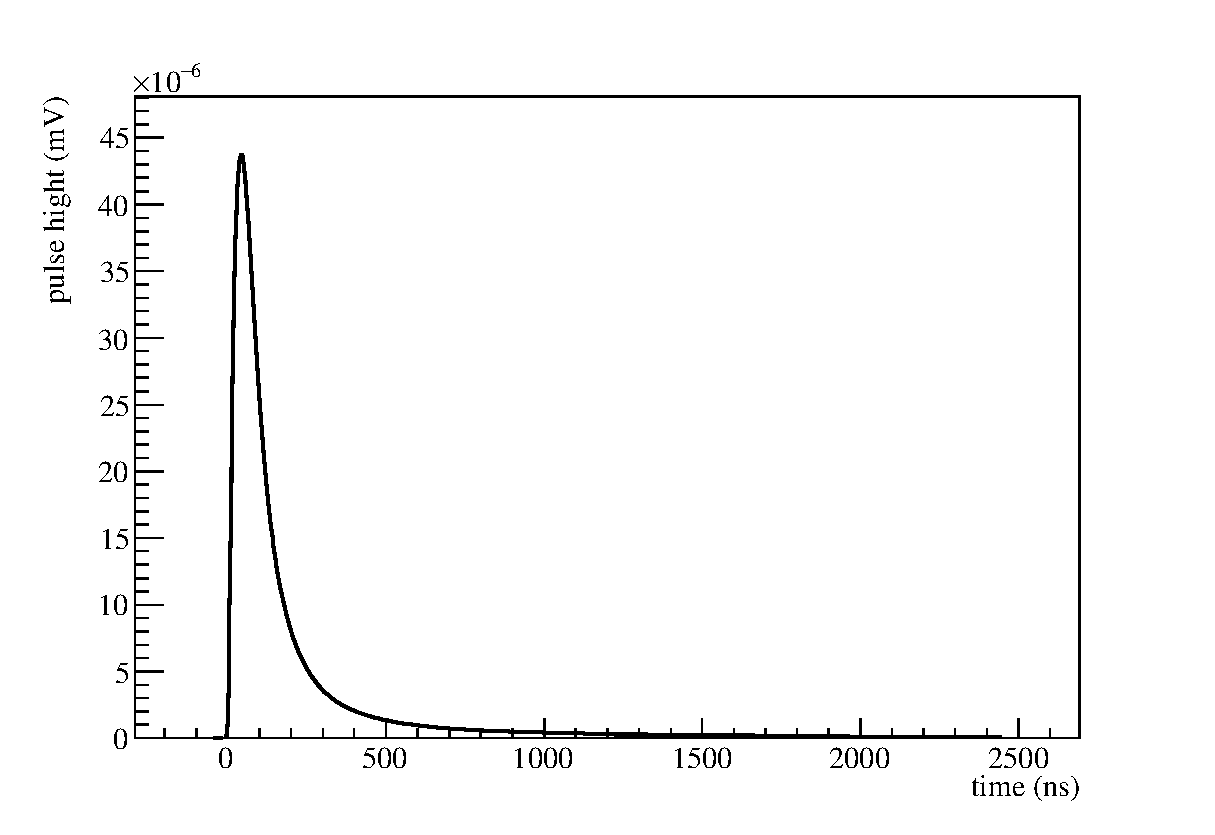
\includegraphics[clip, width=0.9\columnwidth]{waveform.eps}
  \caption{1電子が$\mu$-PICに到達した時に読み出される電気信号.}
  \label{fig::mu-pic_readout}
\end{figure}

\begin{figure}
  \centering
  \begin{subfigure}{0.48\columnwidth}
    \centering
    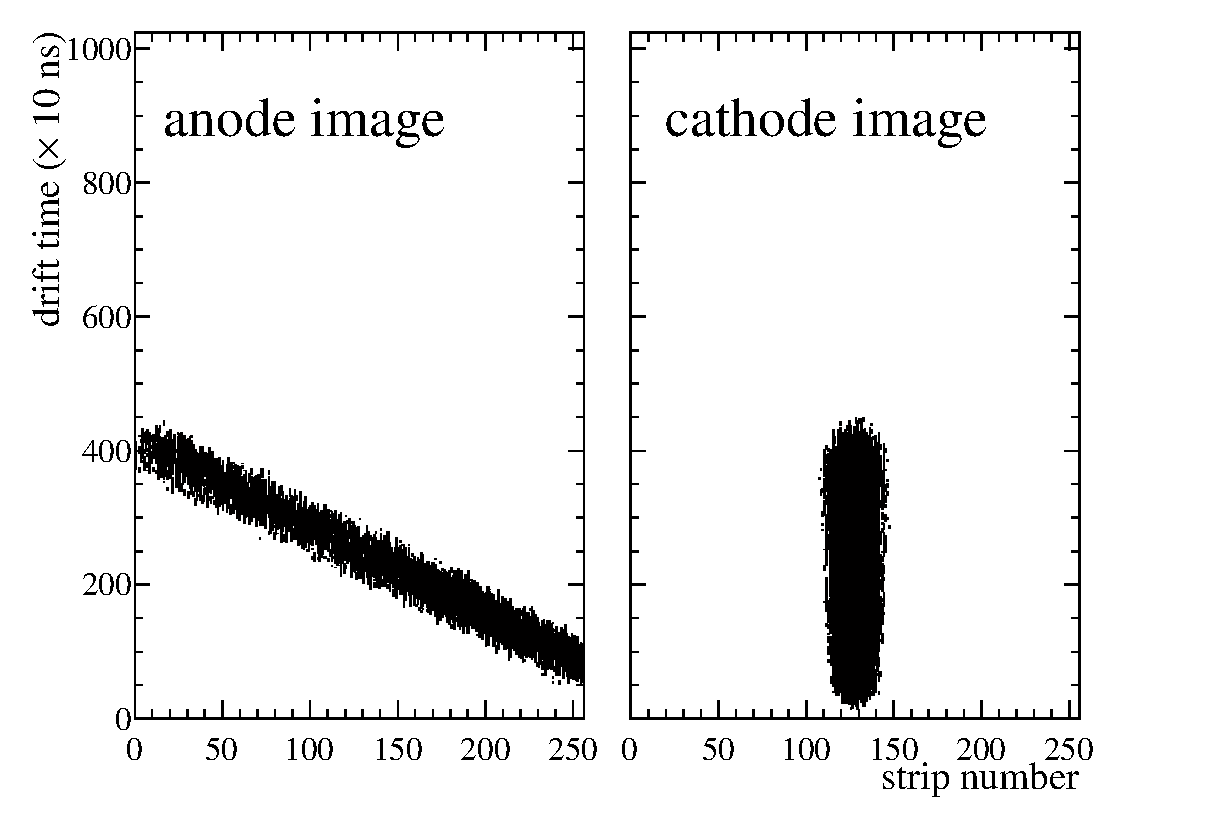
\includegraphics[clip, width=\columnwidth, trim=0 0 50 0]{CH4_0.eps}
    \caption{シミュレーションによるトラック.}
  \end{subfigure}
  \begin{subfigure}{0.48\columnwidth}
    \centering
    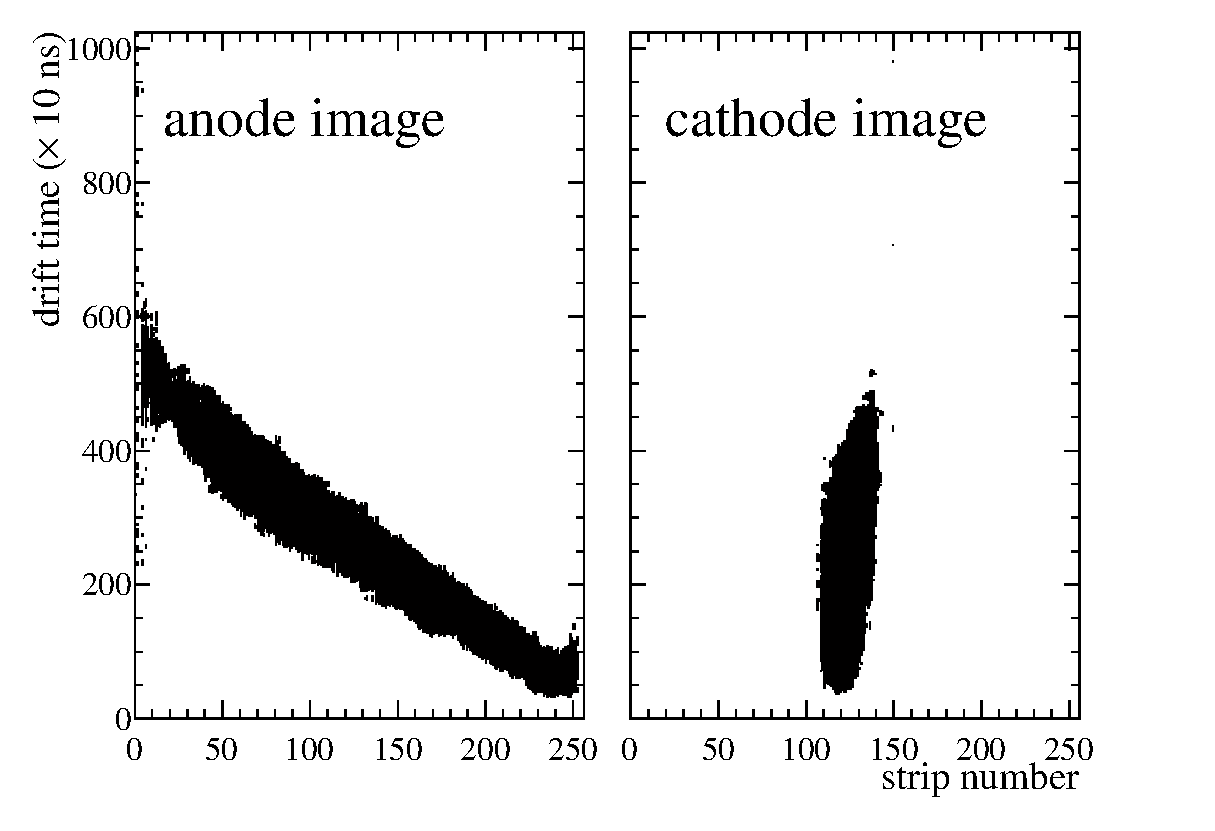
\includegraphics[width=\columnwidth, trim=0 0 50 0]{0160_5.eps}
    \caption{$\alpha$線源によるトラック.}
  \end{subfigure}
  \caption{$\alpha$粒子のトラック(\Methane の場合).}
  \label{fig::track_comp_ch4}
\end{figure}

\begin{figure}
  \centering
  \begin{subfigure}{0.48\columnwidth}
    \centering
    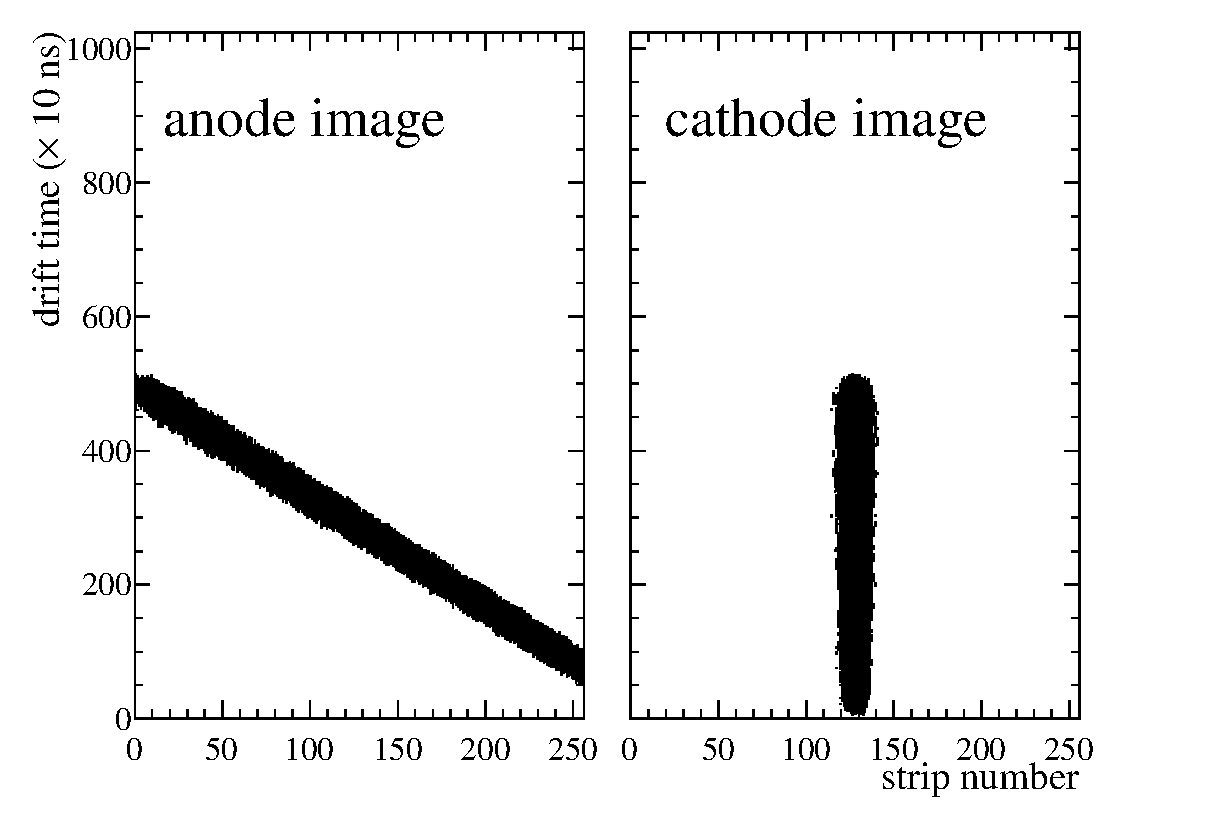
\includegraphics[clip, width=\columnwidth, trim=0 0 50 0]{CH4_3_H2_7_0.eps}
    \caption{シミュレーションによるトラック.}
  \end{subfigure}
  \begin{subfigure}{0.48\columnwidth}
    \centering
    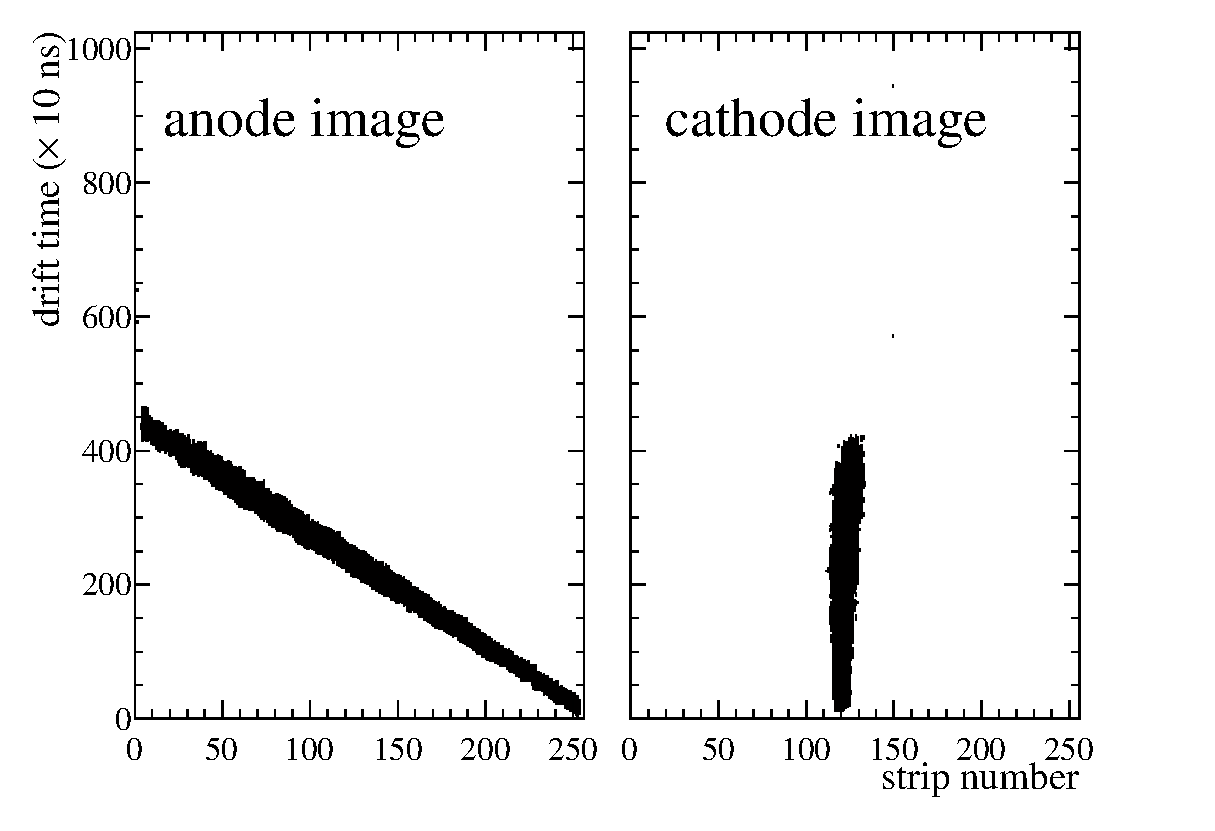
\includegraphics[clip, width=\columnwidth, trim=0 0 50 0]{0207_7.eps}
    \caption{$\alpha$線源によるトラック.}
  \end{subfigure}
  \caption{$\alpha$粒子のトラック(\MethaneHydro の場合).}
  \label{fig::track_comp_ch4_h2}
\end{figure}

\begin{figure}
  \centering
  \begin{subfigure}{0.48\columnwidth}
    \centering
    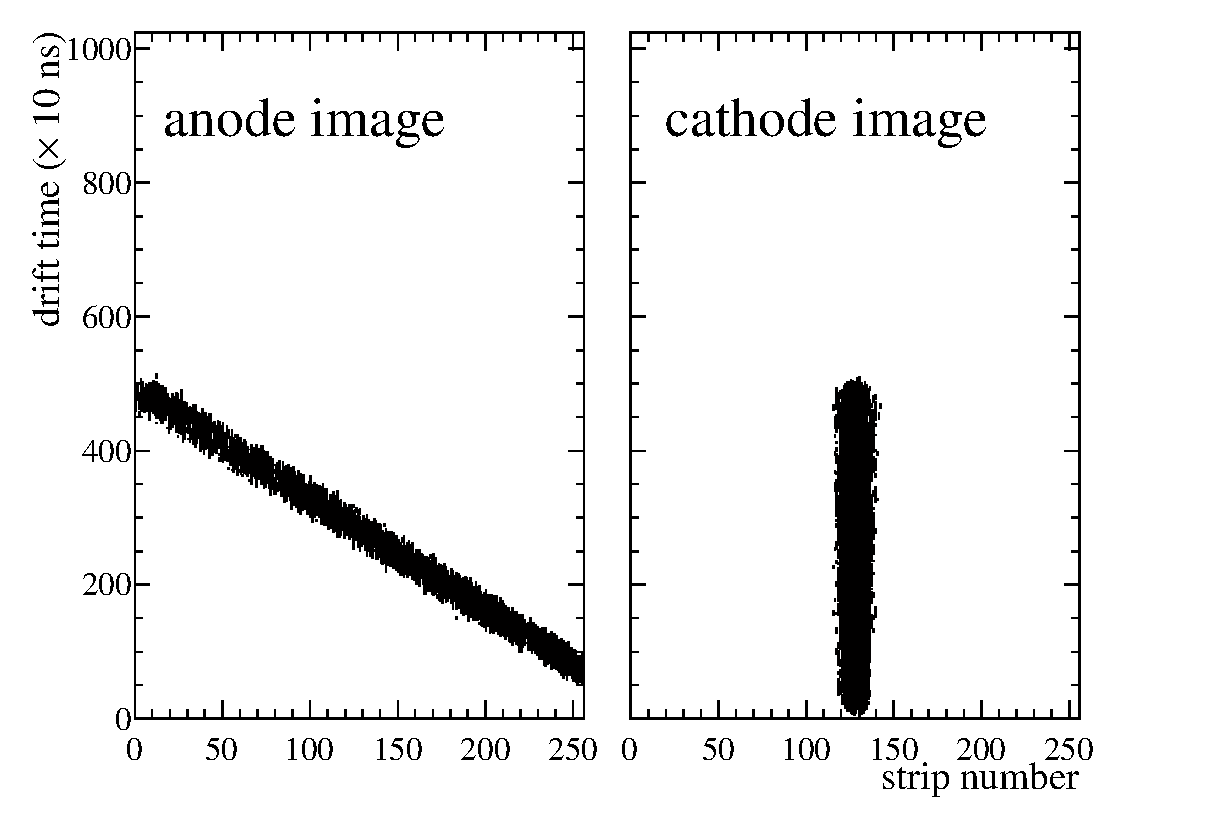
\includegraphics[clip, width=\columnwidth, trim=0 0 50 0]{CH4_4_He_6_0.eps}
    \caption{シミュレーションによるトラック.}
  \end{subfigure}
  \begin{subfigure}{0.48\columnwidth}
    \centering
    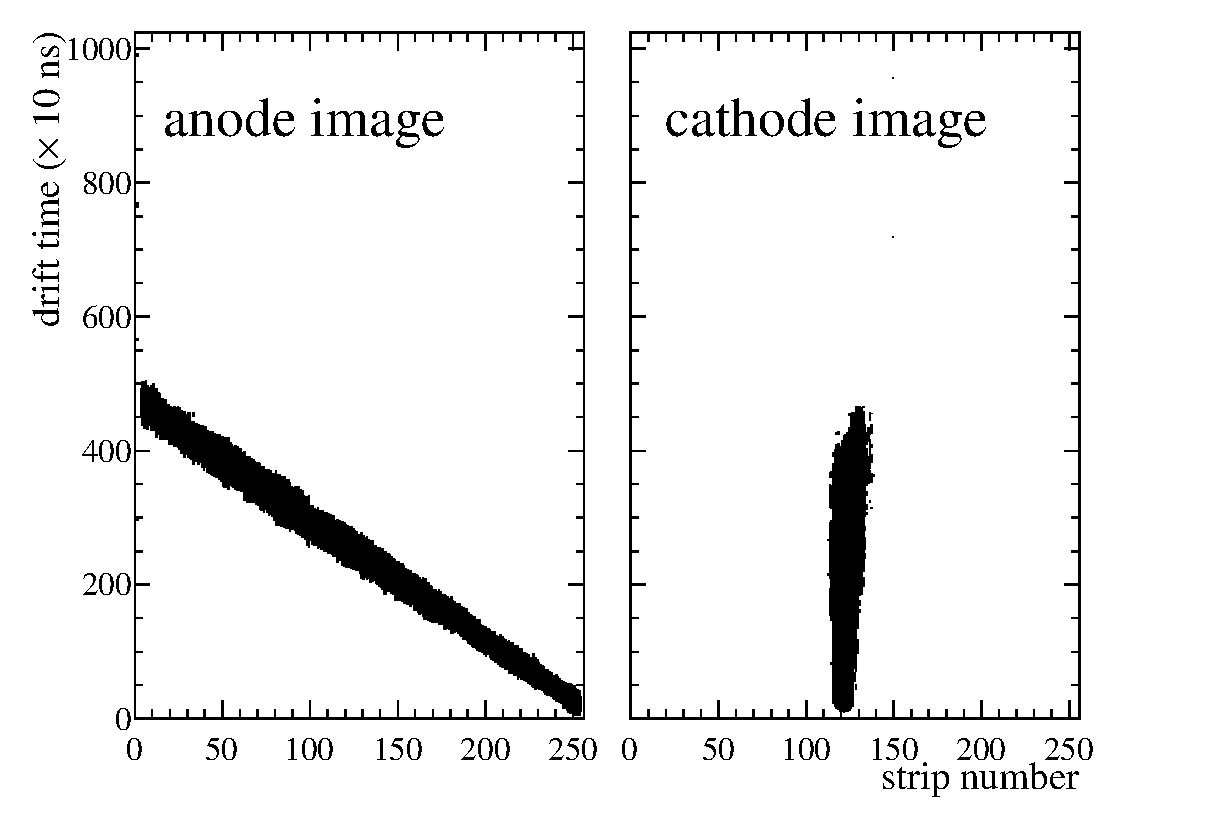
\includegraphics[clip, width=\columnwidth, trim=0 0 50 0]{0163_3.eps}
    \caption{$\alpha$線源によるトラック.}
  \end{subfigure}
  \caption{$\alpha$粒子のトラック(\MethaneHerium の場合).}
  \label{fig::track_comp_ch4_he}
\end{figure}

\begin{figure}
  \centering
  \begin{subfigure}{0.48\columnwidth}
    \centering
    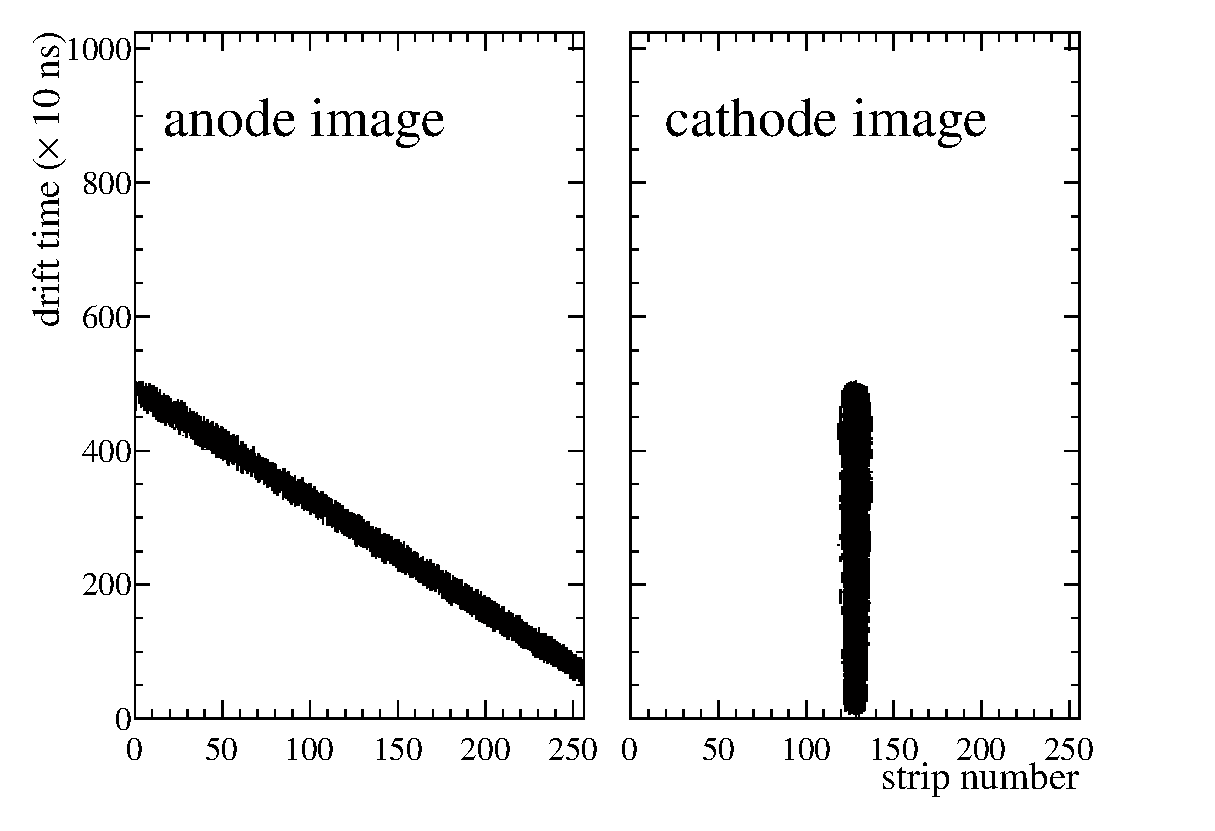
\includegraphics[clip, width=\columnwidth, trim=0 0 50 0]{iC4H10_1_H2_9_0.eps}
    \caption{シミュレーションによるトラック.}
  \end{subfigure}
  \begin{subfigure}{0.48\columnwidth}
    \centering
    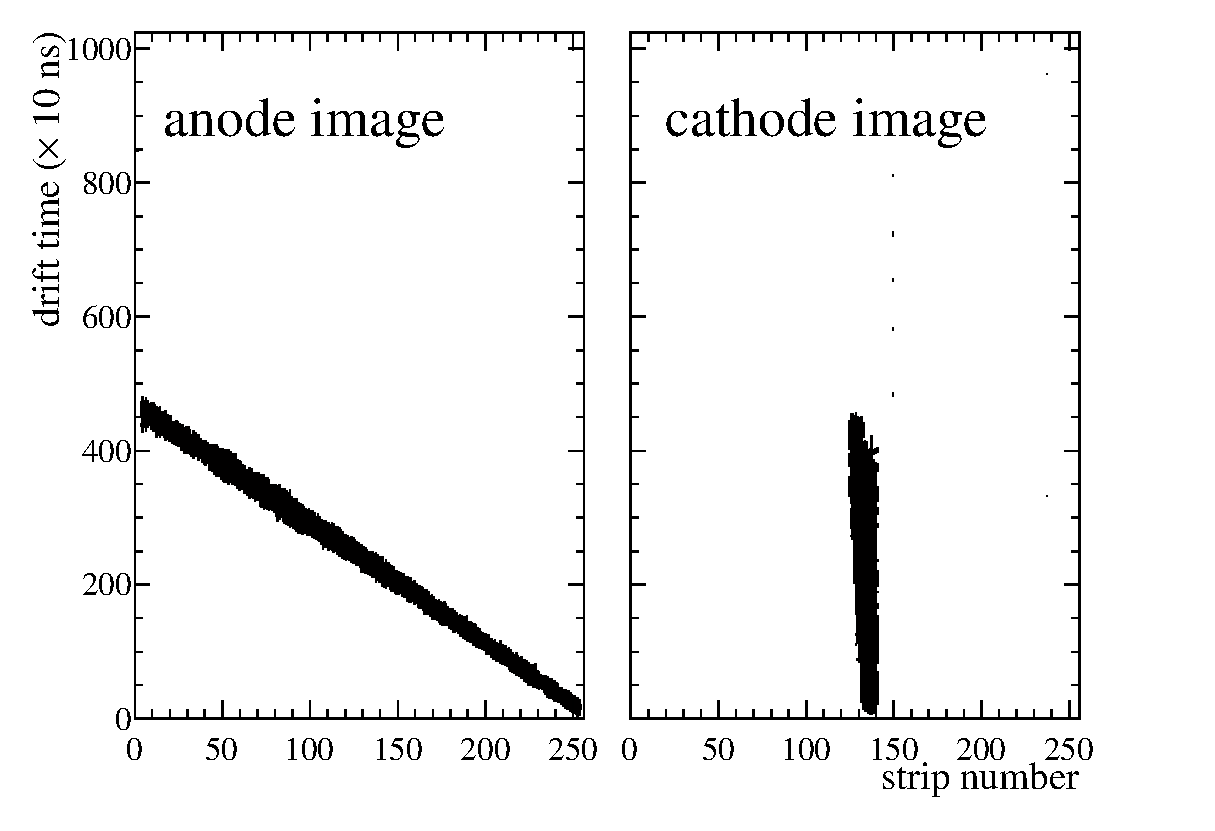
\includegraphics[clip, width=\columnwidth, trim=0 0 50 0]{0210_14.eps}
    \caption{$\alpha$線源によるトラック.}
  \end{subfigure}
  \caption{$\alpha$粒子のトラック(\isoButaneHydro の場合).}
  \label{fig::track_comp_ic4h10_h2}
\end{figure}

\begin{figure}
  \centering
  \begin{subfigure}{0.48\columnwidth}
    \centering
    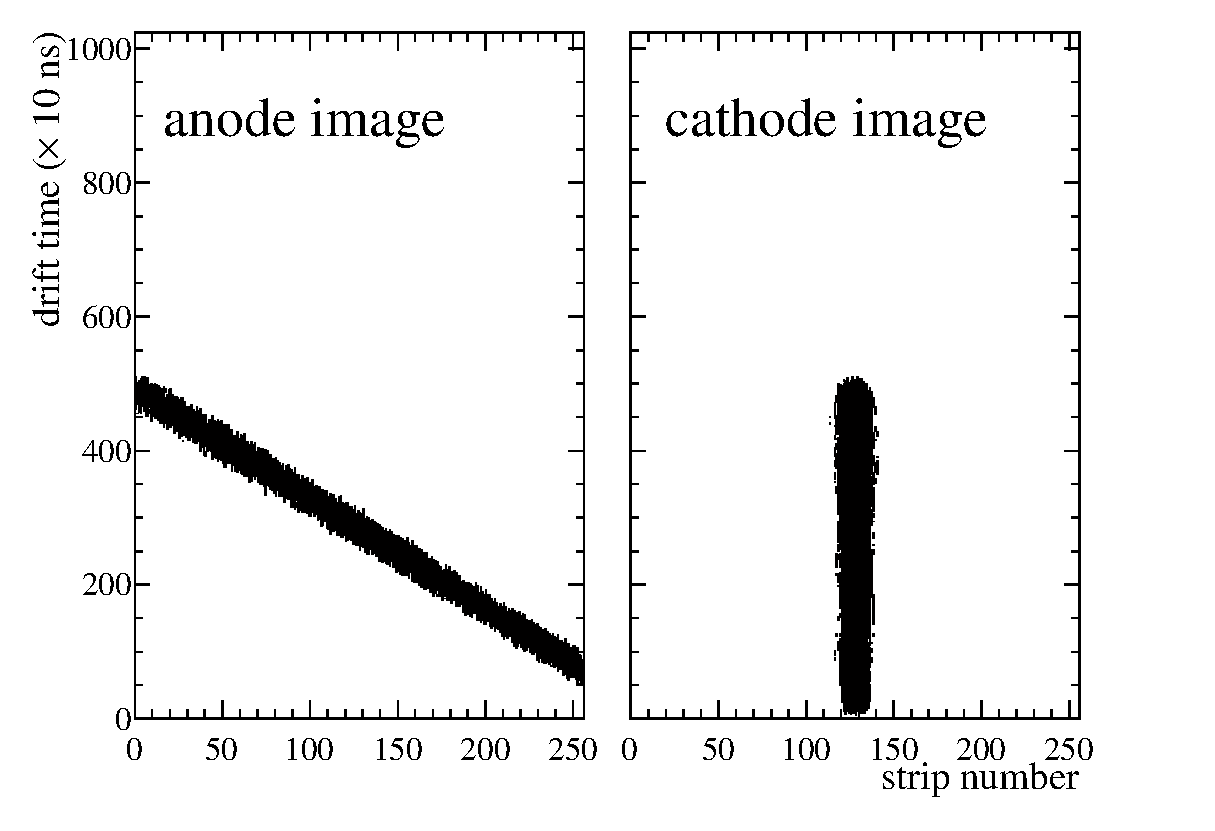
\includegraphics[clip, width=\columnwidth, trim=0 0 50 0]{iC4H10_1_He_9_0.eps}
    \caption{シミュレーションによるトラック.}
  \end{subfigure}
  \begin{subfigure}{0.48\columnwidth}
    \centering
    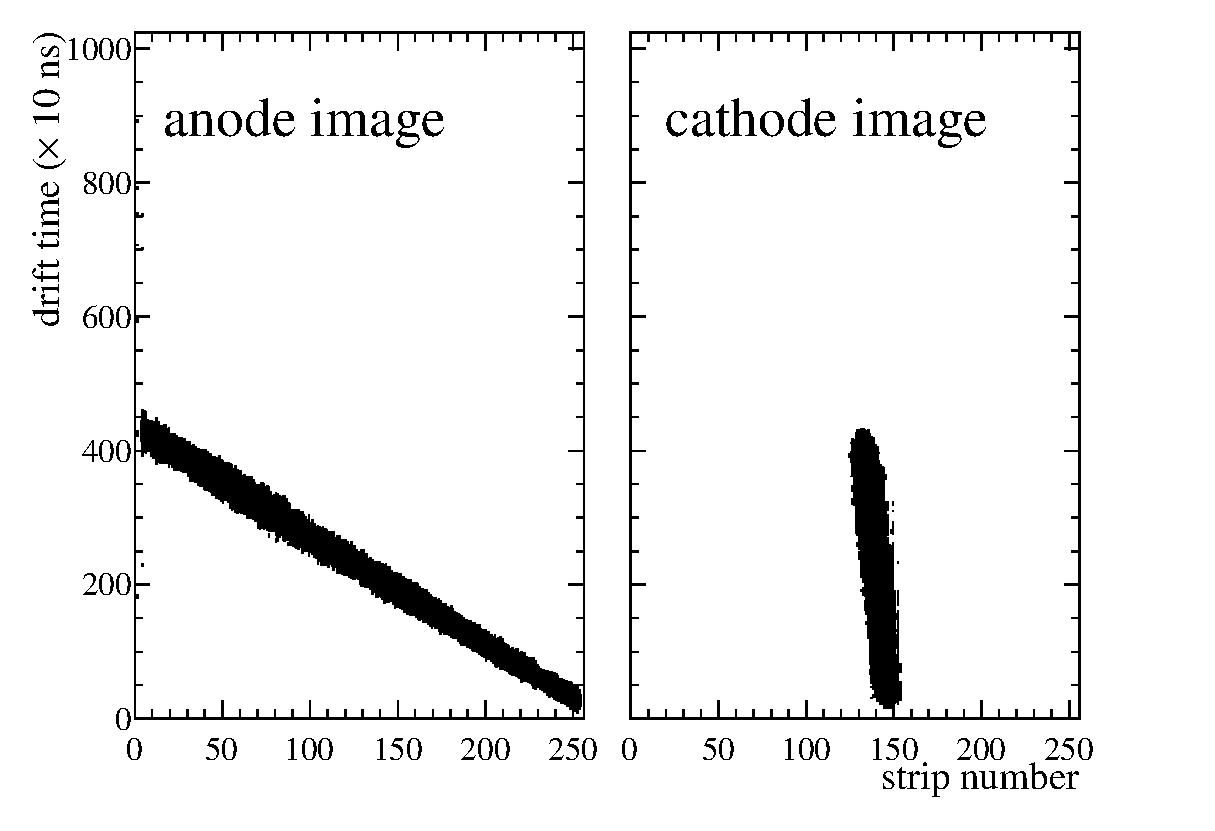
\includegraphics[clip, width=\columnwidth, trim=0 0 50 0]{0176_1.eps}
    \caption{$\alpha$線源によるトラック.}
  \end{subfigure}
  \caption{$\alpha$粒子のトラック(\isoButaneHerium の場合).}
  \label{fig::track_comp_ic4h10_he}
\end{figure}

$\alpha$線源から放出される$\alpha$粒子のエネルギーは\SI{4.2}{\mega\electronvolt}であるが,
実際に測定する$\alpha$粒子のエネルギーは数百\si{\kilo\electronvolt}である.
そこで,$\alpha$線源の前に\SI{15}{\micro\metre}のカプトンを挟むことで$\alpha$粒子のエネルギーを落として測定を行った.
有感領域と線源の間にある検出ガスによってエネルギーを落とし約\SI{1}{\mega\electronvolt}となる.
図\ref{fig::track_ch4_loss},\ref{fig::track_ch4_h2_loss},\ref{fig::track_ch4_he_loss},
\ref{fig::track_ic4h10_h2_loss},\ref{fig::track_ic4h10_he_loss}に示す.
コリメータの\ang{30}の穴を用いたため,斜めのトラックとなっている.
シミュレーションでは有感領域の横から\SI{500}{\kilo\electronvolt}の$\alpha$粒子を飛ばした.
$\alpha$線源から放出されるエネルギーに広がりがあるため,
エネルギーを完全に合わせていないが,トラックの傾向は再現できている.
\begin{figure}
  \centering
  \begin{subfigure}{0.48\columnwidth}
    \centering
    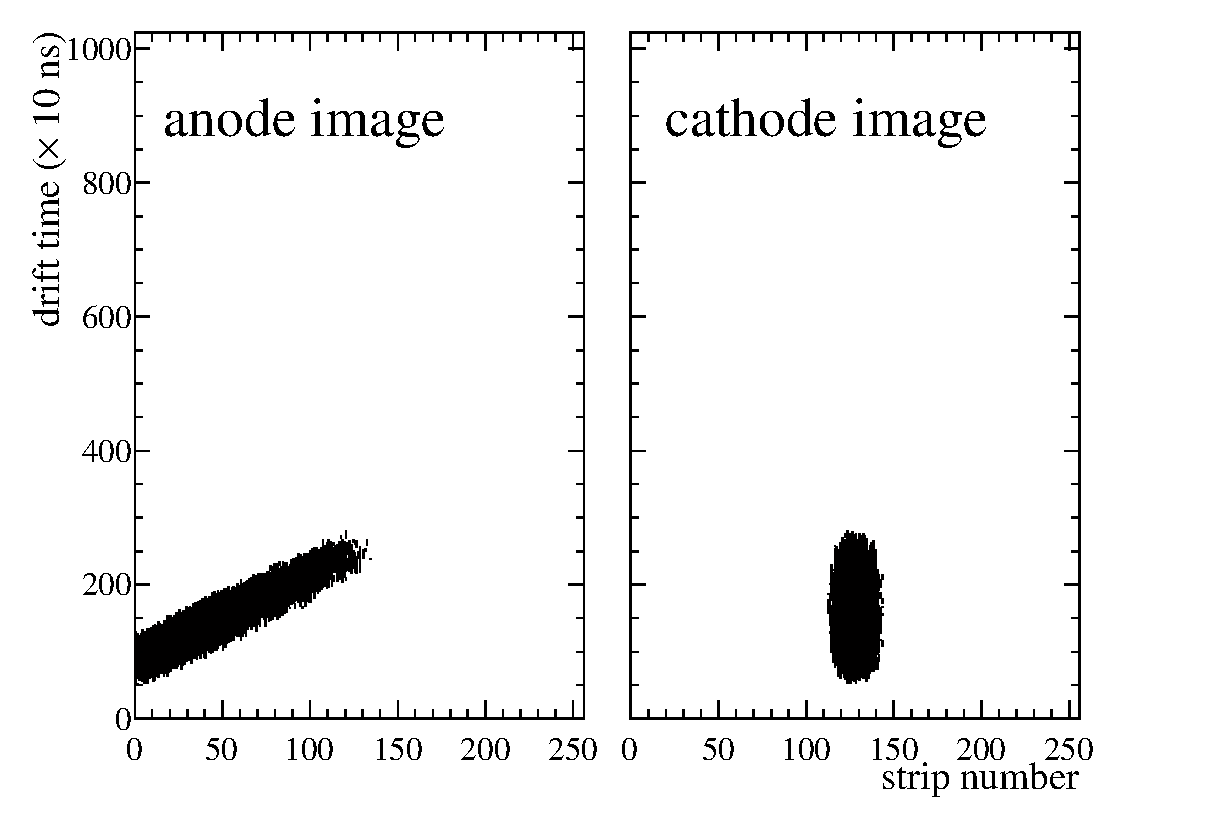
\includegraphics[clip, width=\columnwidth, trim=0 0 50 0]{a_source_CH4_50_nostr_3.eps}
    \caption{シミュレーションによるトラック.}
  \end{subfigure}
  \begin{subfigure}{0.48\columnwidth}
    \centering
    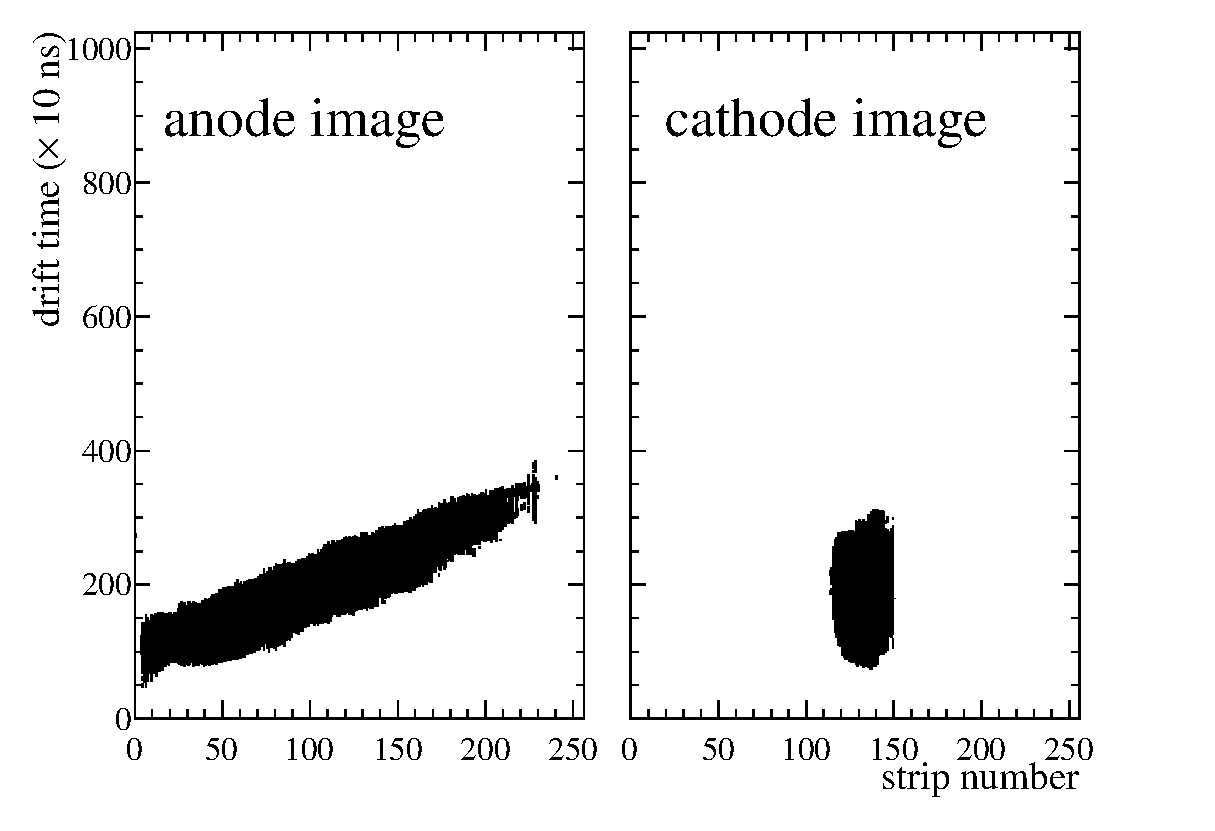
\includegraphics[clip, width=\columnwidth, trim=0 0 50 0]{0146_16.eps}
    \caption{$\alpha$線源によるトラック.}
  \end{subfigure}
  \caption{低エネルギー$\alpha$粒子のトラック(\Methane の場合).}
  \label{fig::track_ch4_loss}
\end{figure}
\begin{figure}
  \centering
  \begin{subfigure}{0.48\columnwidth}
    \centering
    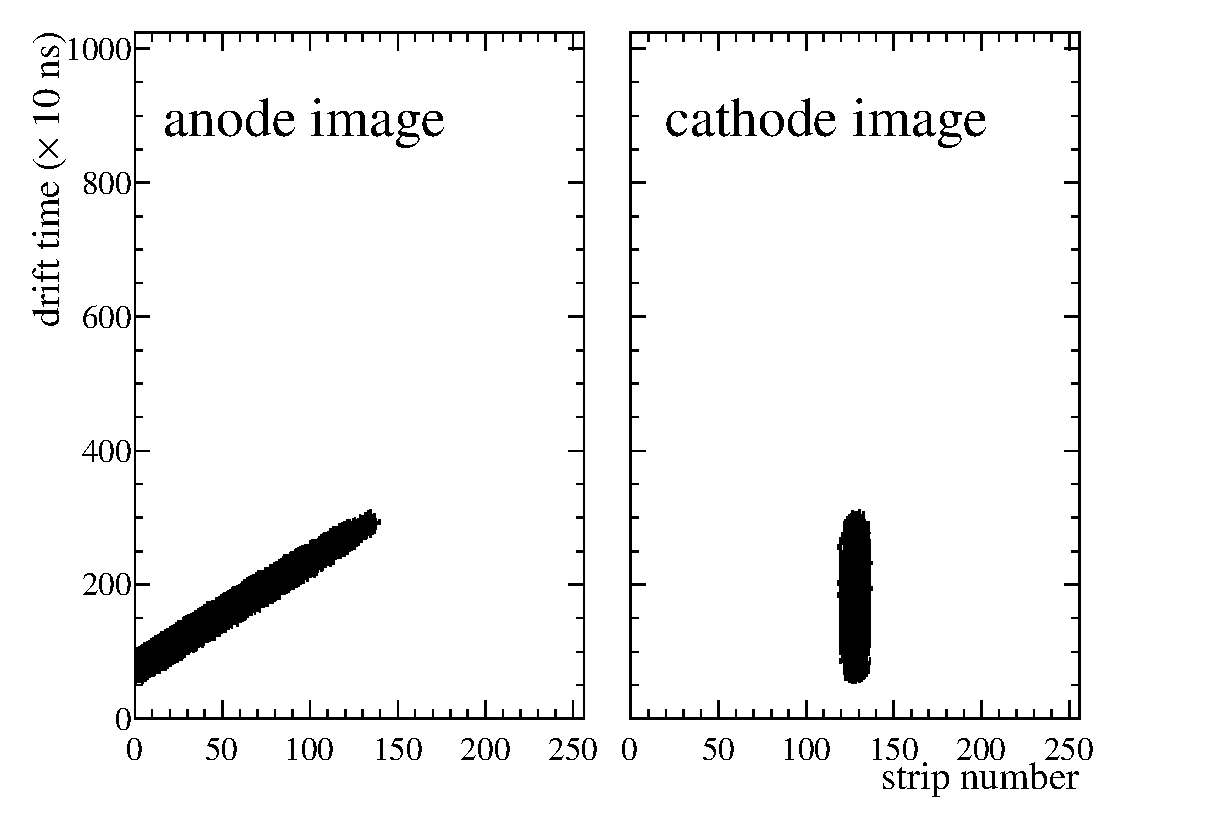
\includegraphics[clip, width=\columnwidth, trim=0 0 50 0]{a_source_CH4_3_H2_7_100_nostr_0.eps}
    \caption{シミュレーションによるトラック.}
  \end{subfigure}
  \begin{subfigure}{0.48\columnwidth}
    \centering
    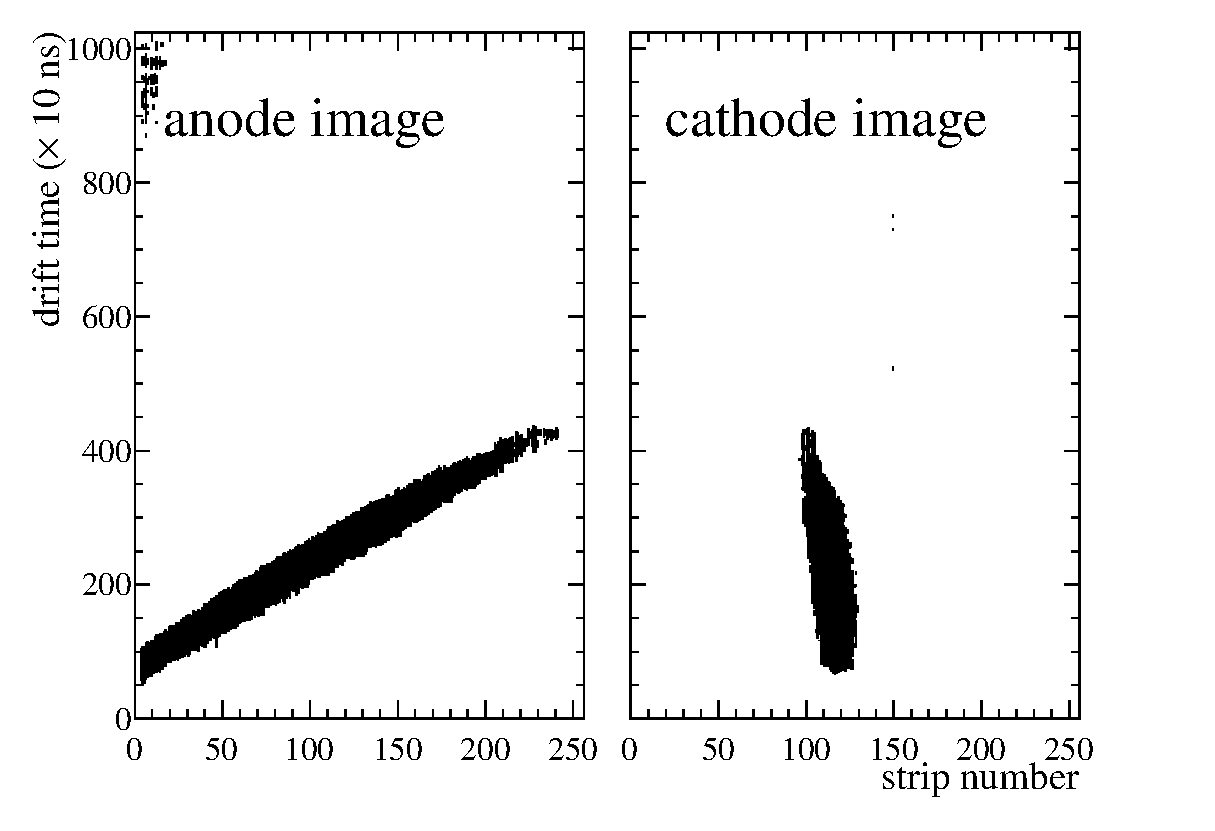
\includegraphics[clip, width=\columnwidth, trim=0 0 50 0]{0209_22.eps}
    \caption{$\alpha$線源によるトラック.}
  \end{subfigure}
  \caption{低エネルギー$\alpha$粒子のトラック(\MethaneHydro の場合).}
  \label{fig::track_ch4_h2_loss}
\end{figure}
\begin{figure}
  \centering
  \begin{subfigure}{0.48\columnwidth}
    \centering
    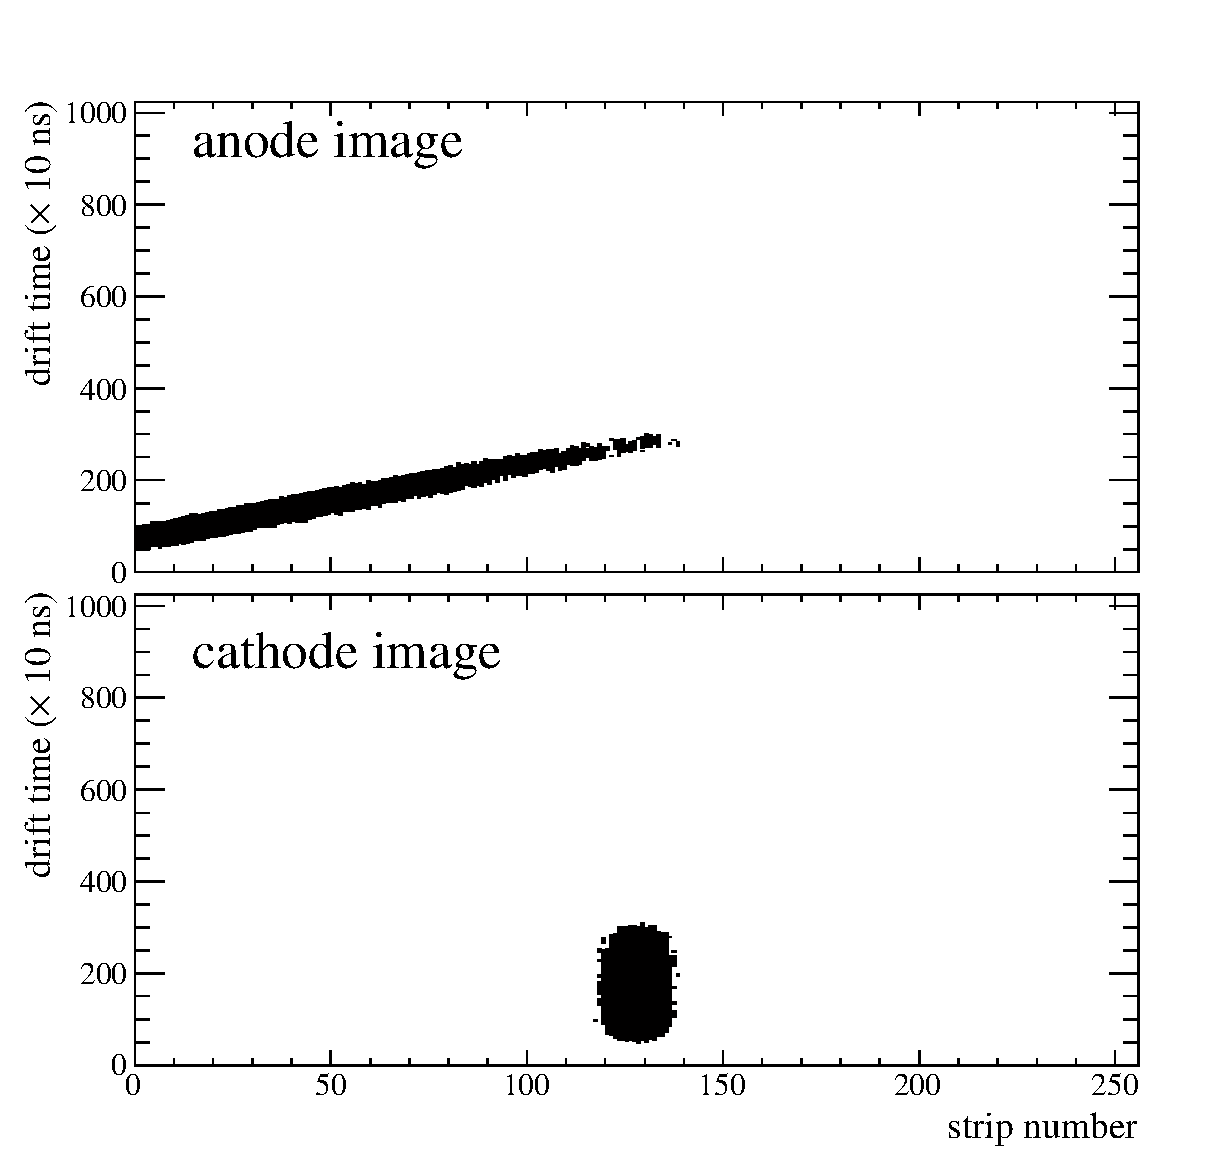
\includegraphics[clip, width=\columnwidth, trim=0 0 50 0]{a_source_CH4_4_He_6_100_nostr_0.eps}
    \caption{シミュレーションによるトラック.}
  \end{subfigure}
  \begin{subfigure}{0.48\columnwidth}
    \centering
    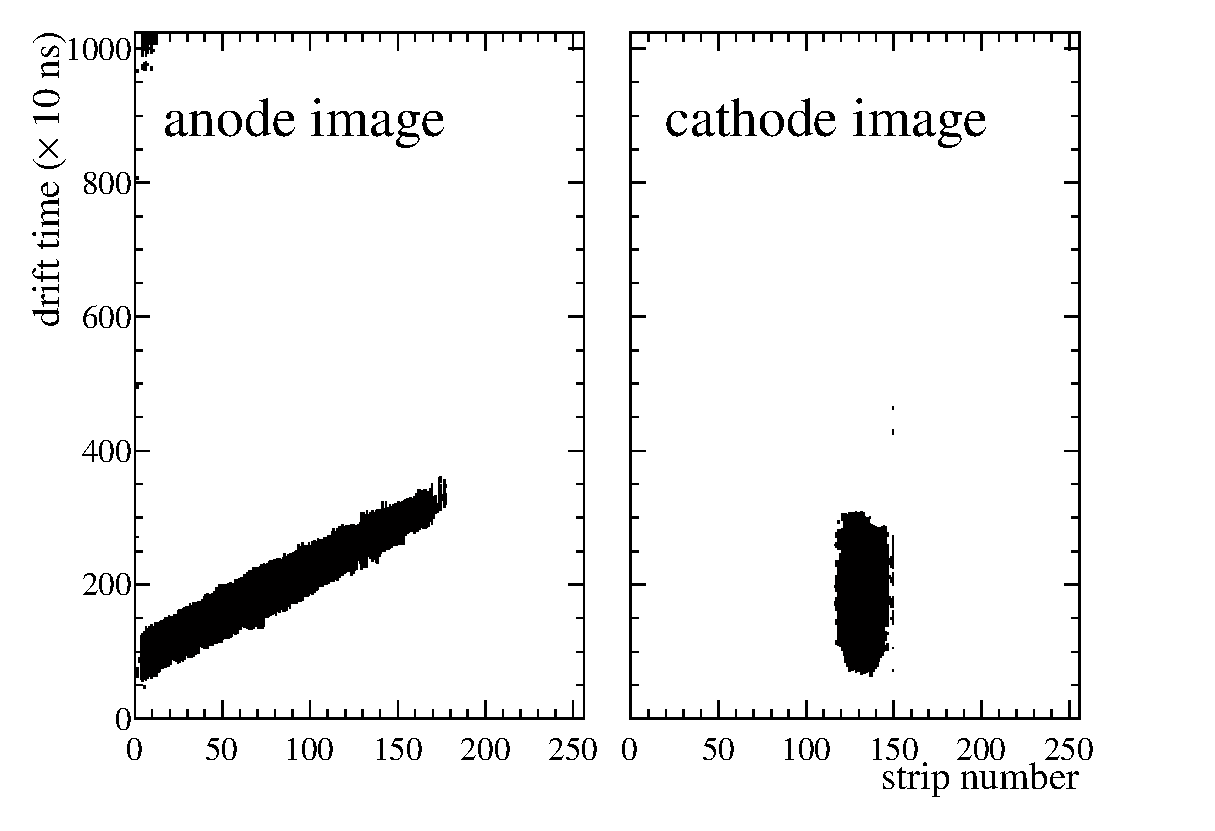
\includegraphics[clip, width=\columnwidth, trim=0 0 50 0]{0204_24.eps}
    \caption{$\alpha$線源によるトラック.}
  \end{subfigure}
  \caption{低エネルギー$\alpha$粒子のトラック(\MethaneHerium の場合).}
  \label{fig::track_ch4_he_loss}
\end{figure}
\begin{figure}
  \centering
  \begin{subfigure}{0.48\columnwidth}
    \centering
    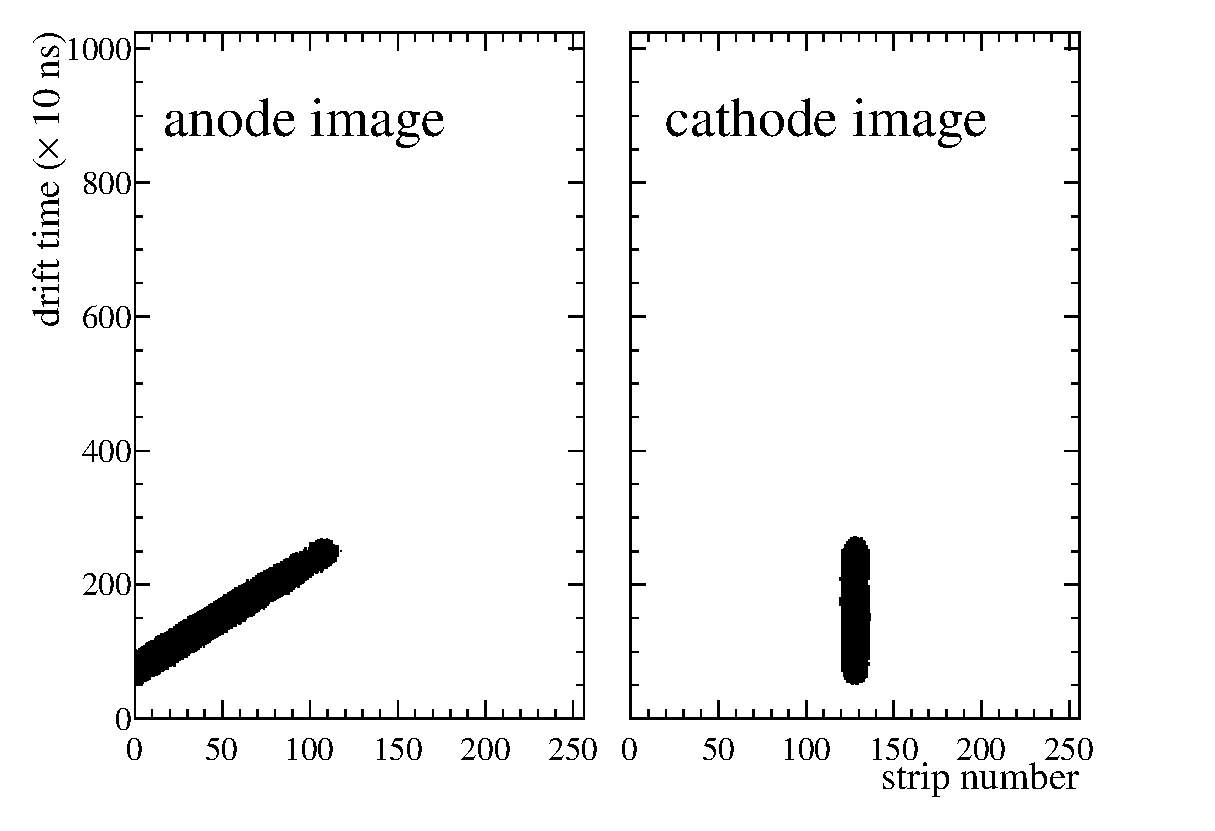
\includegraphics[clip ,width=\columnwidth, trim=0 0 50 0]{a_source_iC4H10_1_H2_9_100_nostr_1.eps}
    \caption{シミュレーションによるトラック.}
  \end{subfigure}
  \begin{subfigure}{0.48\columnwidth}
    \centering
    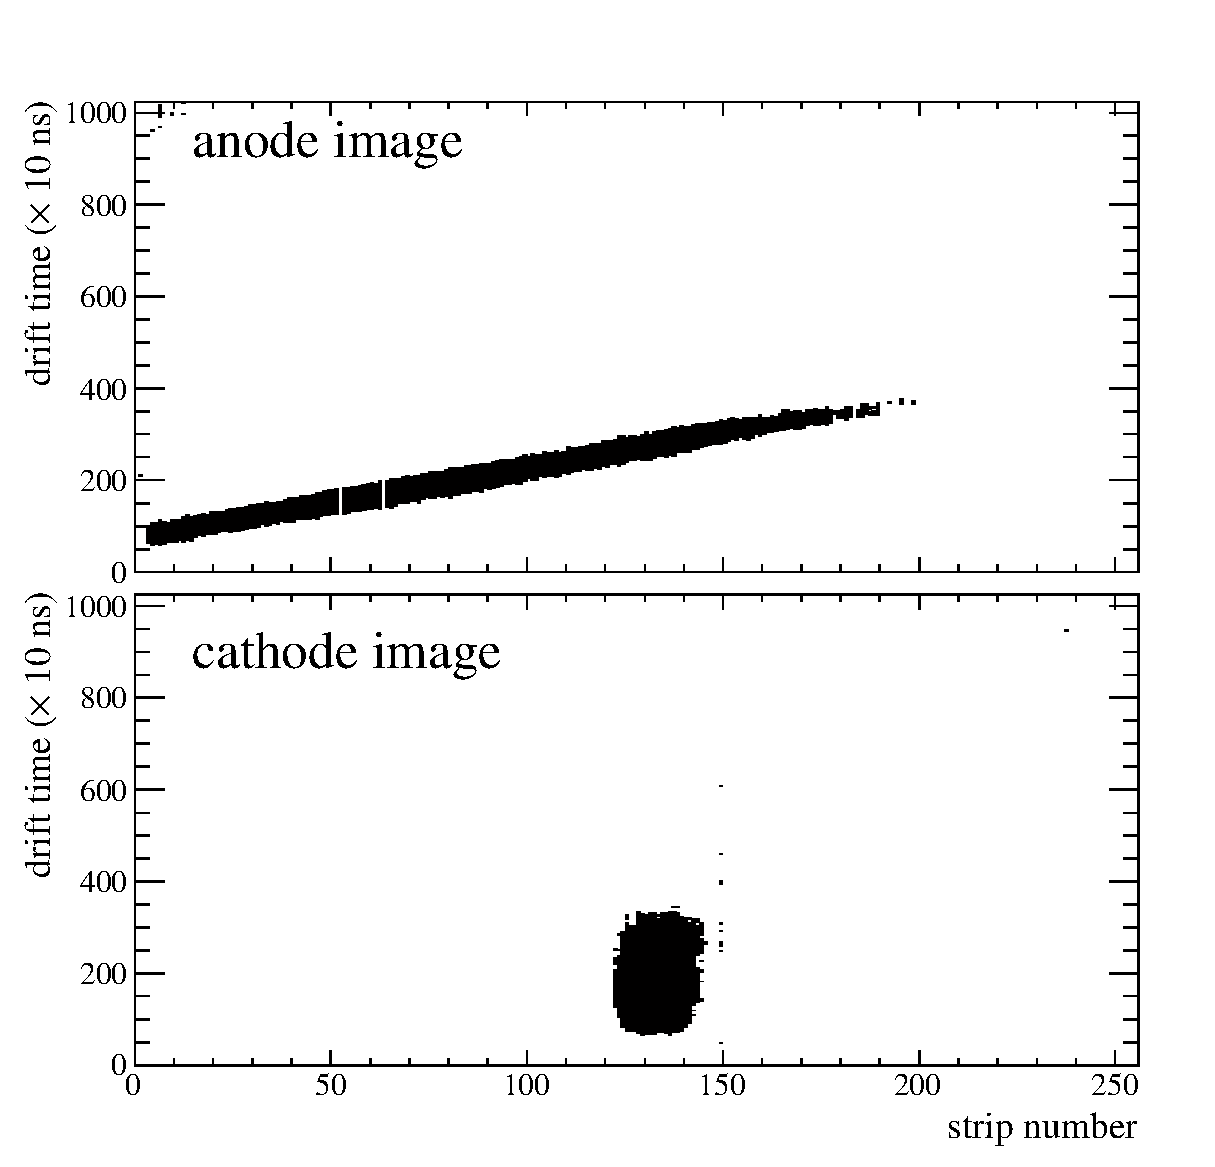
\includegraphics[clip, width=\columnwidth, trim=0 0 50 0]{0211_4.eps}
    \caption{$\alpha$線源によるトラック.}
  \end{subfigure}
  \caption{低エネルギー$\alpha$粒子のトラック(\isoButaneHydro の場合).}
  \label{fig::track_ic4h10_h2_loss}
\end{figure}
\begin{figure}
  \centering
  \begin{subfigure}{0.48\columnwidth}
    \centering
    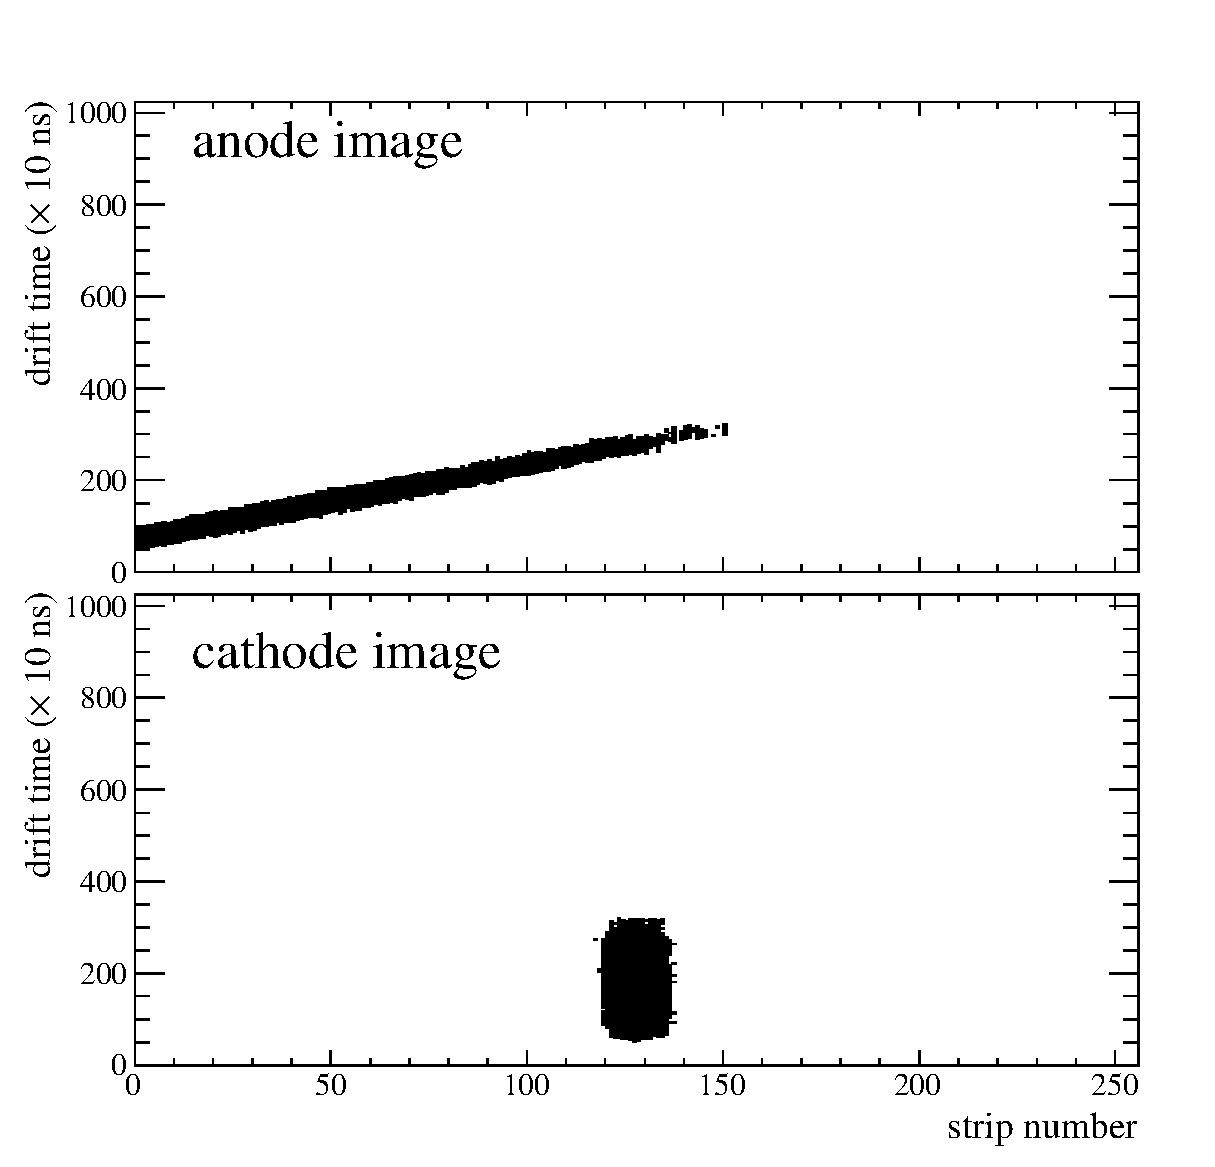
\includegraphics[clip, width=\columnwidth, trim=0 0 50 0]{a_source_iC4H10_1_He_9_100_nostr_0.eps}
    \caption{シミュレーションによるトラック.}
  \end{subfigure}
  \begin{subfigure}{0.48\columnwidth}
    \centering
    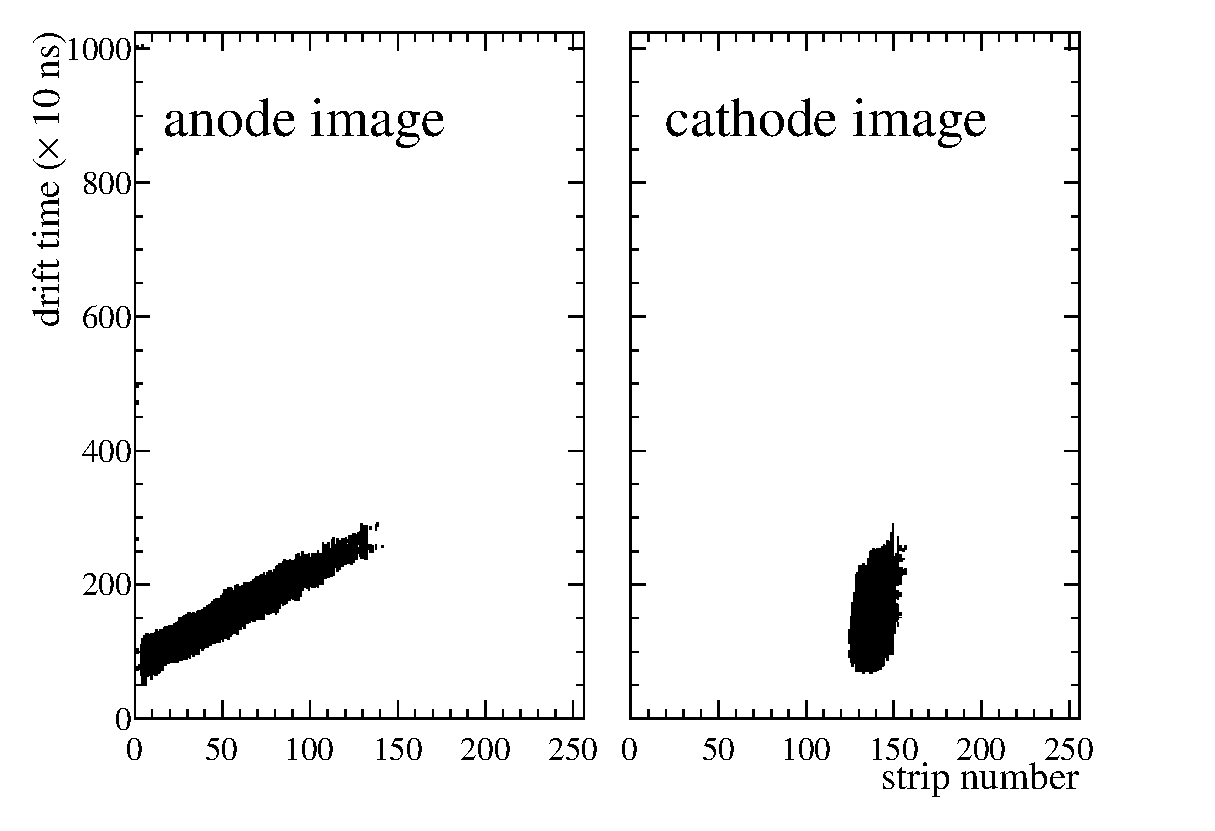
\includegraphics[clip, width=\columnwidth, trim=0 0 50 0]{0203_10.eps}
    \caption{$\alpha$線源によるトラック.}
  \end{subfigure}
  \caption{低エネルギー$\alpha$粒子のトラック(\isoButaneHerium の場合).}
  \label{fig::track_ic4h10_he_loss}
\end{figure}

\section{トリプルアルファ反応のシミュレーション}
\label{sec::triple_alpha_simulation}
$\alpha$線源のトラックを再現することができたので,
同じ設定で${}^{12}{\mathrm{C}}({\mathrm{n}},{\mathrm{n}}')3\alpha$のシミュレーションを行う.
このシミュレーションでは以下のように3つの$\alpha$粒子を生成した.
\begin{enumerate}
\item
  ${}^{12}\mathrm{C}$が\SI{14}{\mega\electronvolt}の中性子との散乱により$0_2^+$状態に励起させる.
  この際,重心系で一様な散乱角で散乱させる.
\item
  ${}^{12}\mathrm{C} (0_2^+)$を$\alpha$粒子と${}^{8}\mathrm{Be}$に位相空間で一様に崩壊させる.
\item
  崩壊してできた${}^{8}\mathrm{Be}$を2つの$\alpha$粒子に位相空間で一様に崩壊させる.
\end{enumerate}
このようにして生成した$\alpha$粒子のトラックを生成する.
トラックの生成方法は前節で述べた通りである.
生成したトラックを図\ref{fig::three_alpha_ch4}, \ref{fig::three_alpha_ch4_h2}, \ref{fig::three_alpha_ch4_he},
\ref{fig::three_alpha_ic4h10_h2}, \ref{fig::three_alpha_ic4h10_he}に示す.
ここでは,3つのトラックを確認できたイベントを選んで示した.
\begin{figure}
  \centering
  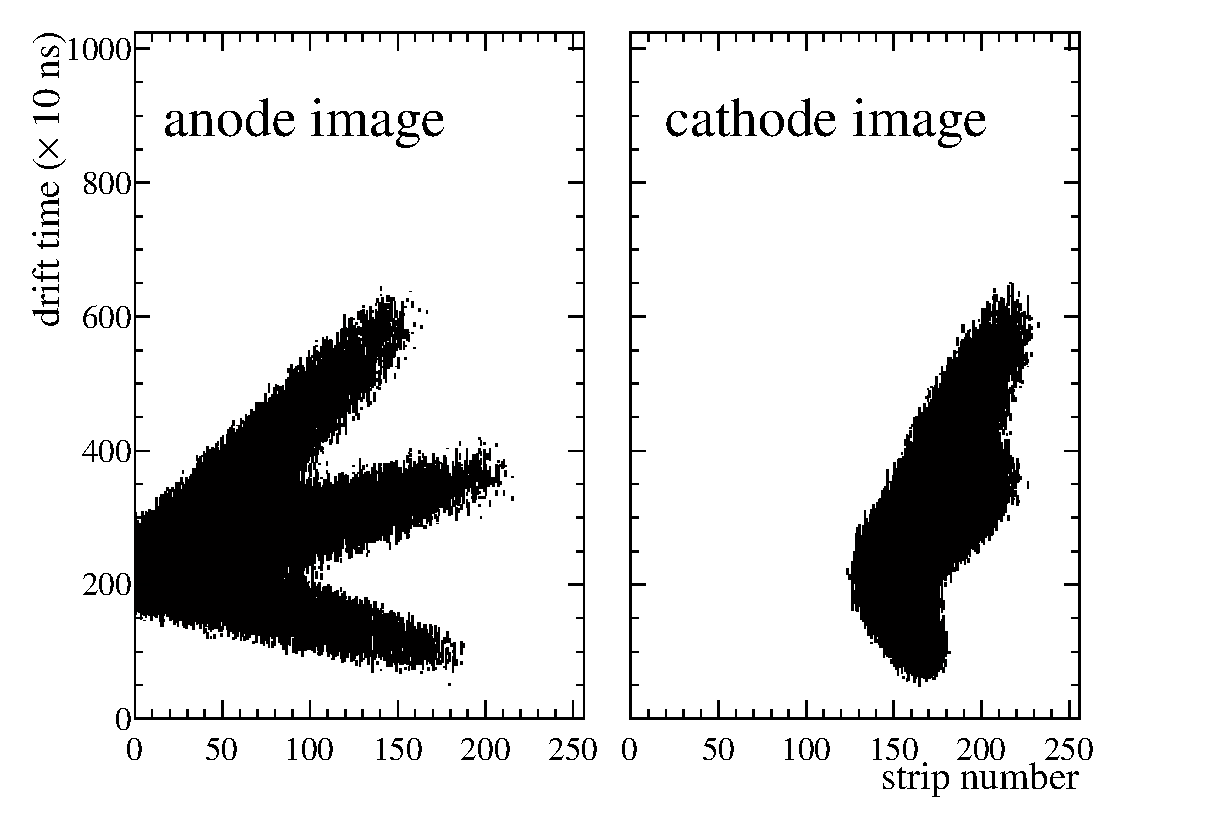
\includegraphics[clip, width=0.8\columnwidth]{10020_7.eps}
  \caption{3$\alpha$のシミュレーション画像 (\Methane の場合).}
  \label{fig::three_alpha_ch4}
\end{figure}

\begin{figure}
  \centering
  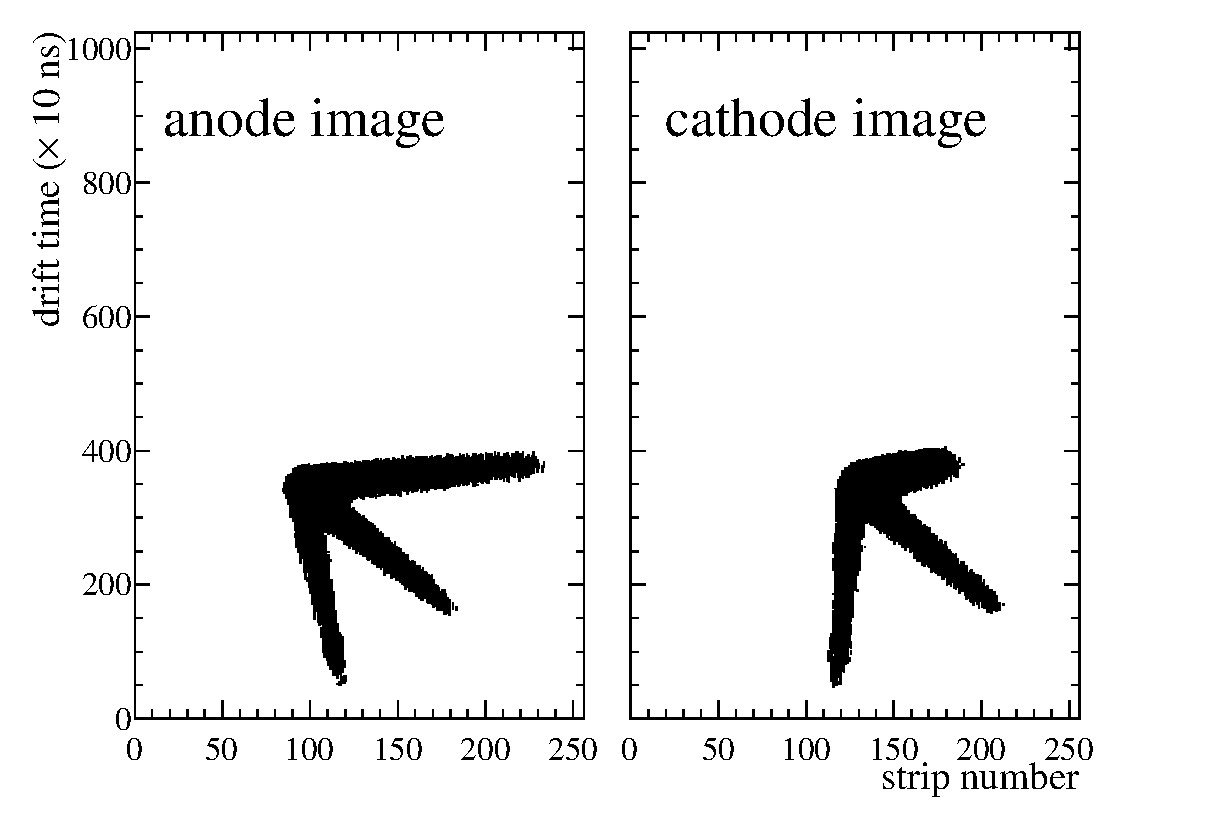
\includegraphics[clip, width=0.8\columnwidth]{10022_15.eps}
  \caption{3$\alpha$のシミュレーション画像 (\MethaneHydro の場合).}
  \label{fig::three_alpha_ch4_h2}
\end{figure}

\begin{figure}
  \centering
  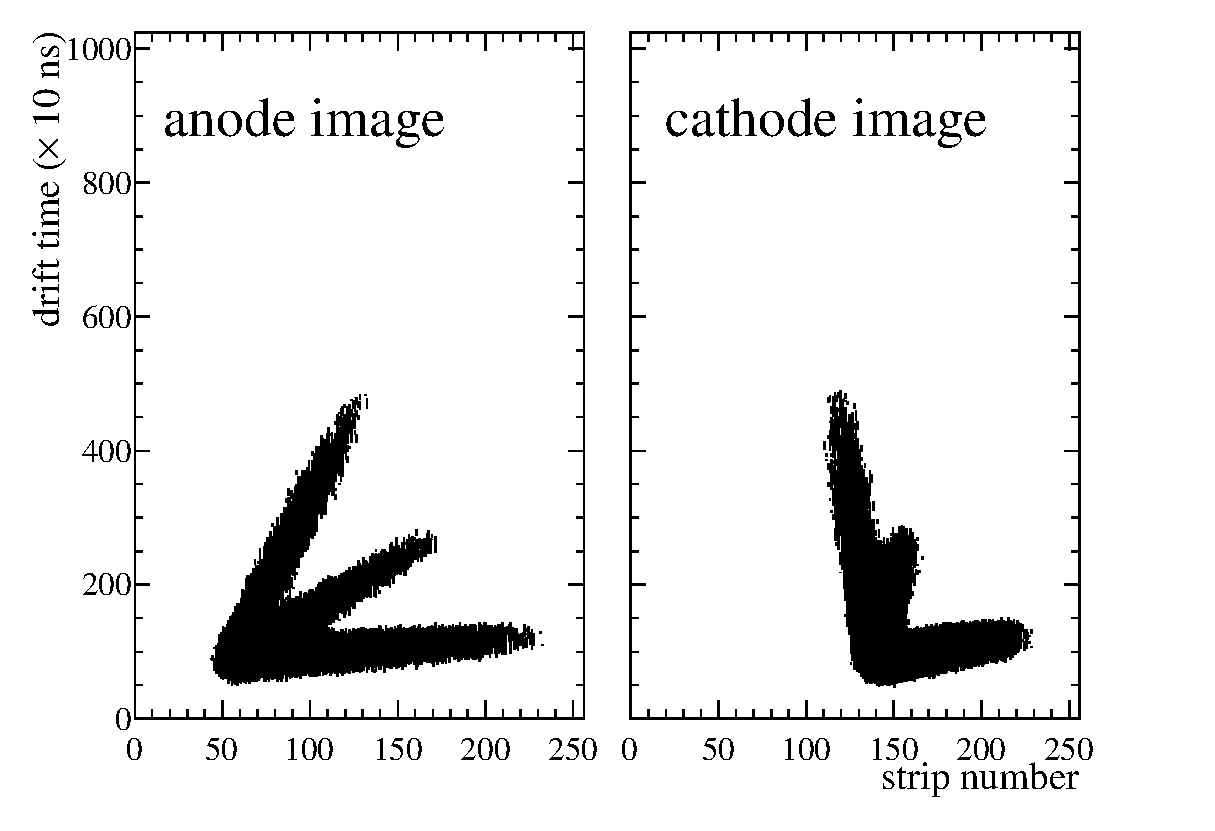
\includegraphics[clip, width=0.8\columnwidth]{10021_5.eps}
  \caption{3$\alpha$のシミュレーション画像 (\MethaneHerium の場合).}
  \label{fig::three_alpha_ch4_he}
\end{figure}

\begin{figure}
  \centering
  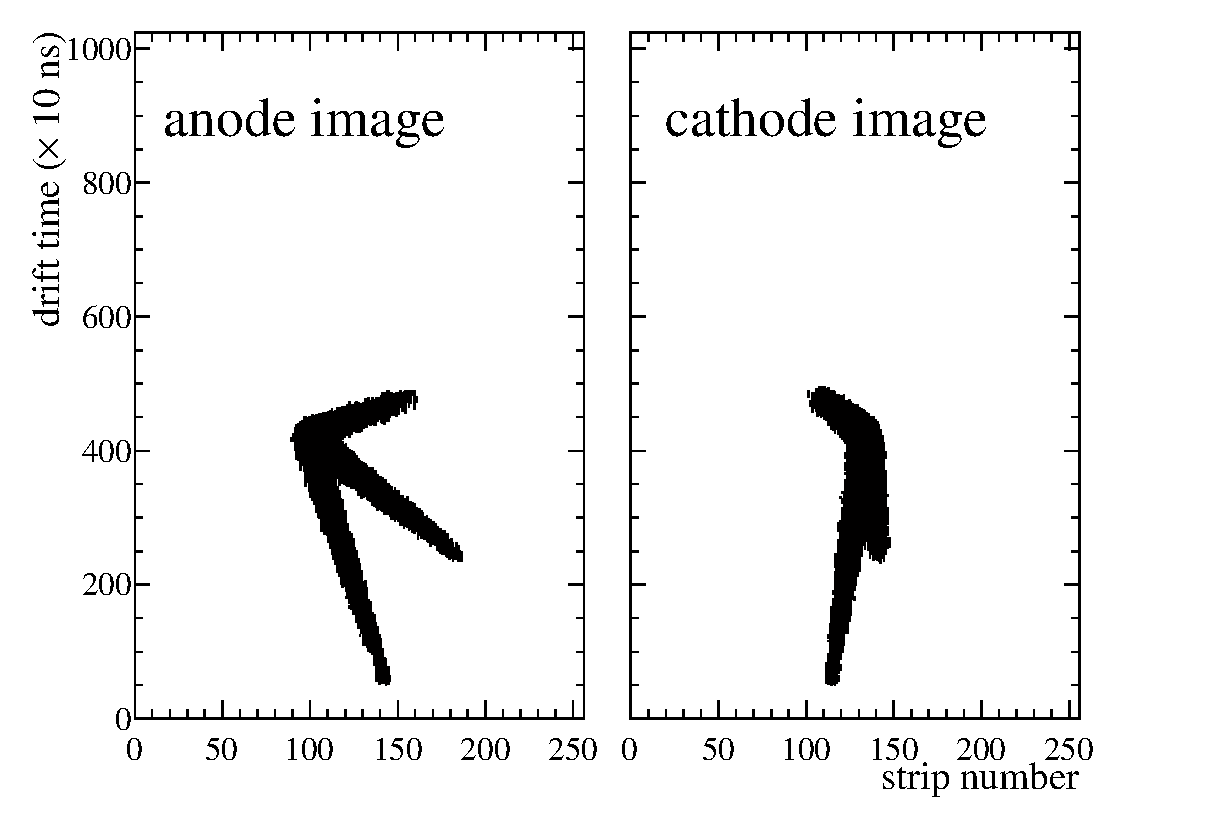
\includegraphics[clip, width=0.8\columnwidth]{10024_9.eps}
  \caption{3$\alpha$のシミュレーション画像 (\isoButaneHydro の場合).}
  \label{fig::three_alpha_ic4h10_h2}
\end{figure}

\begin{figure}
  \centering
  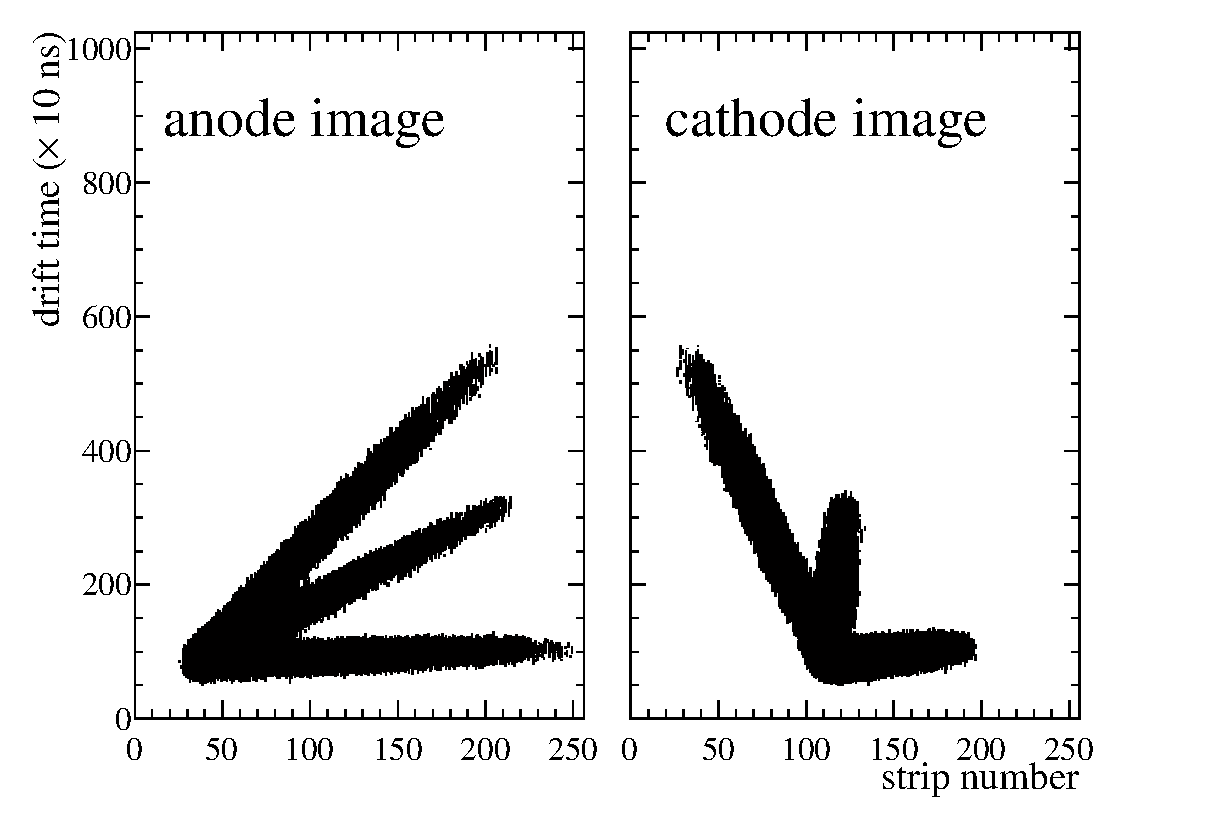
\includegraphics[clip, width=0.8\columnwidth]{10023_0.eps}
  \caption{3$\alpha$のシミュレーション画像 (\isoButaneHerium の場合).}
  \label{fig::three_alpha_ic4h10_he}
\end{figure}

生成されたイベントの中には3本のトラックを確認できないイベントも含まれている.
図\ref{fig::not_three_alpha_ch4},\ref{fig::not_three_alpha_ch4_h2},\ref{fig::not_three_alpha_ch4_he},
\ref{fig::not_three_alpha_ic4h10_h2},\ref{fig::not_three_alpha_ic4h10_he}にそのような例を示す.
\begin{figure}
  \centering
  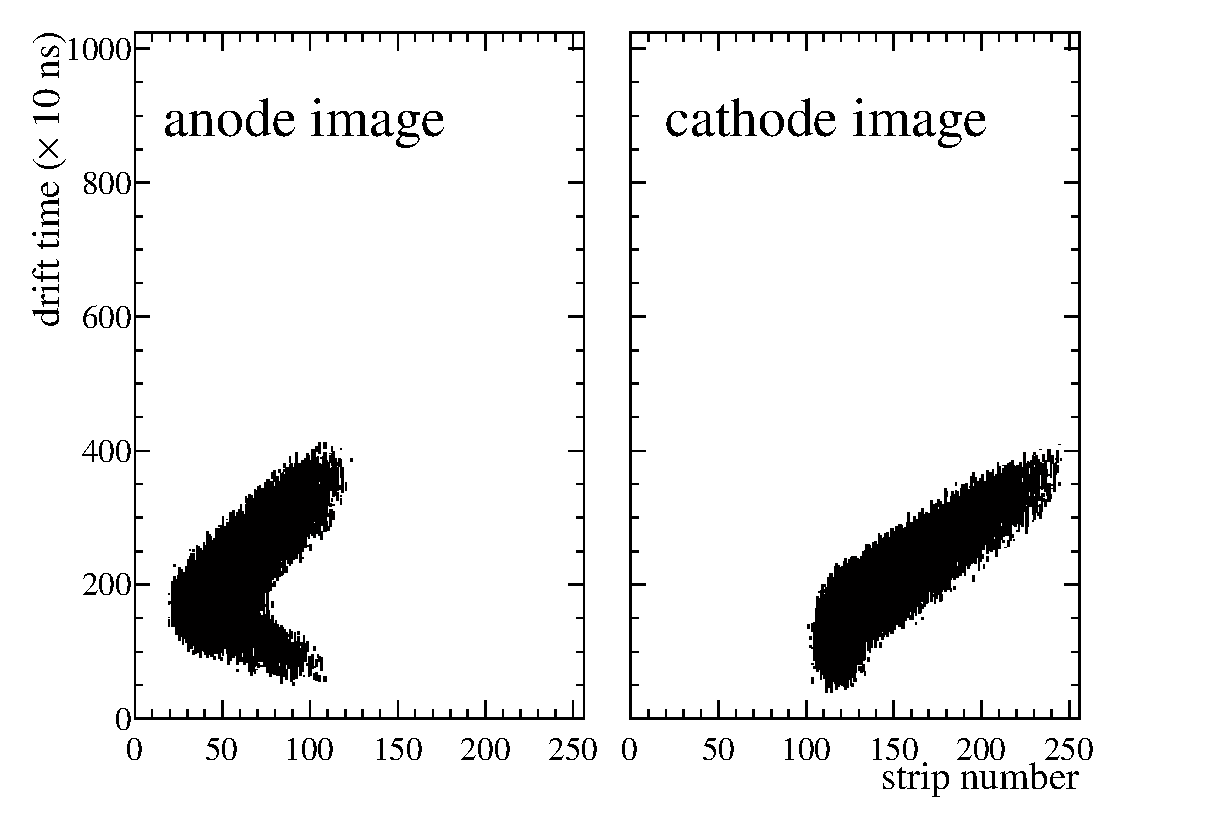
\includegraphics[clip, width=0.8\columnwidth]{10020_5.eps}
  \caption{2本しかトラックを確認できないイベントの画像 (\Methane の場合).}
  \label{fig::not_three_alpha_ch4}
\end{figure}
\begin{figure}
  \centering
  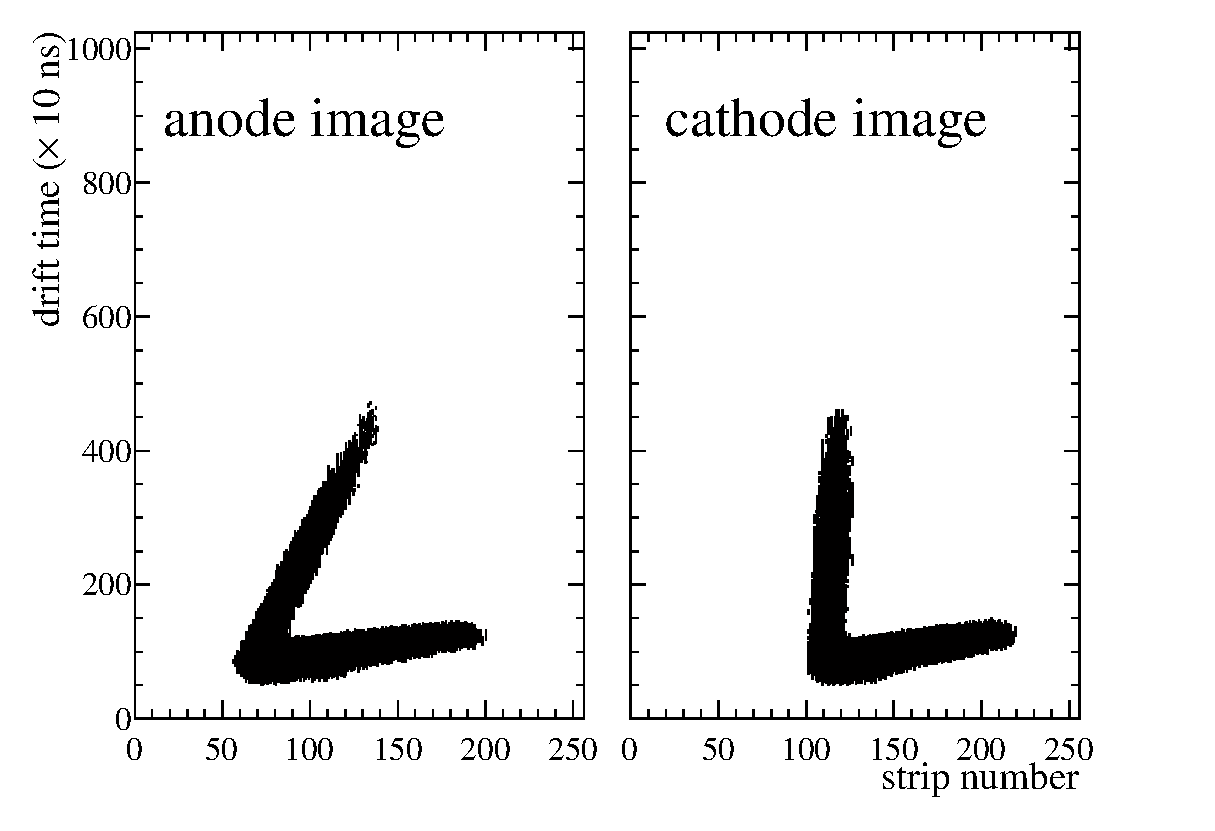
\includegraphics[clip, width=0.8\columnwidth]{10022_49.eps}
  \caption{2本しかトラックを確認できないイベントの画像 (\MethaneHydro の場合).}
  \label{fig::not_three_alpha_ch4_h2}
\end{figure}
\begin{figure}
  \centering
  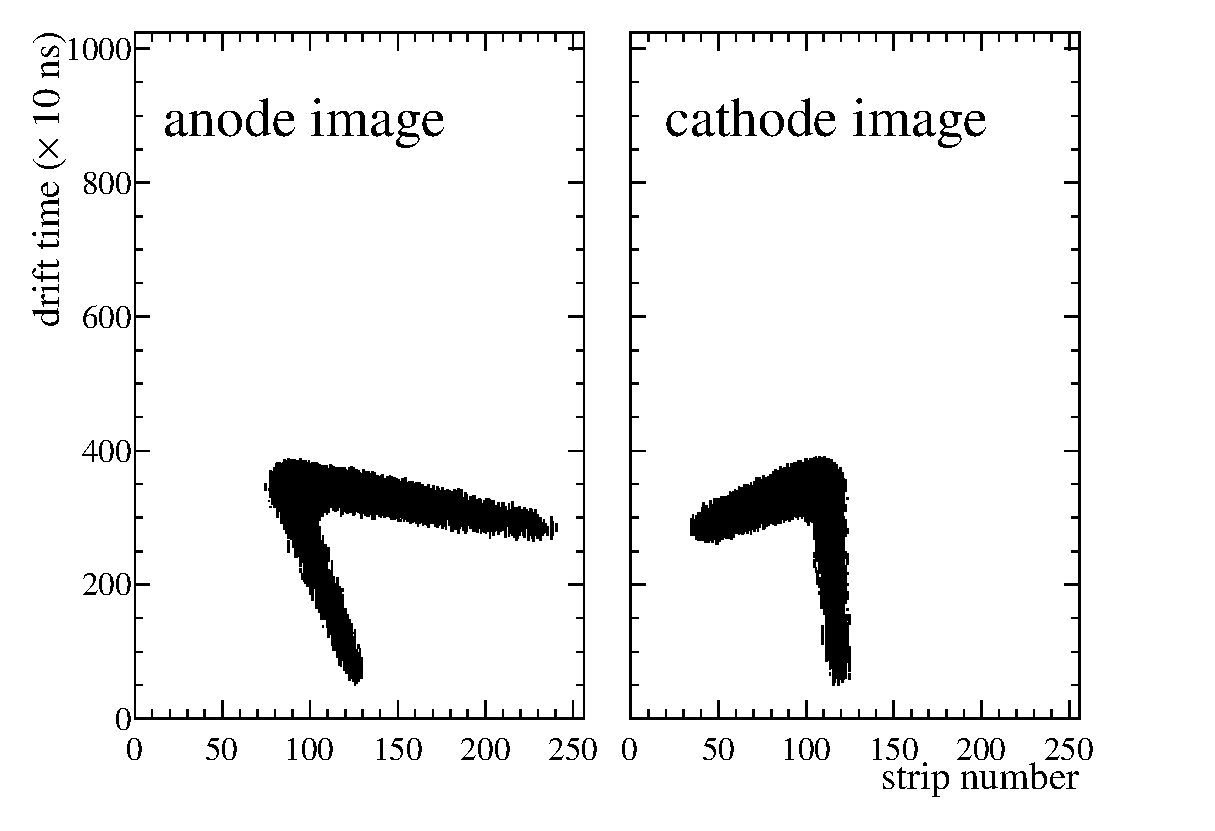
\includegraphics[clip, width=0.8\columnwidth]{10021_24.eps}
  \caption{2本しかトラックを確認できないイベントの画像 (\MethaneHerium の場合).}
  \label{fig::not_three_alpha_ch4_he}
\end{figure}
\begin{figure}
  \centering
  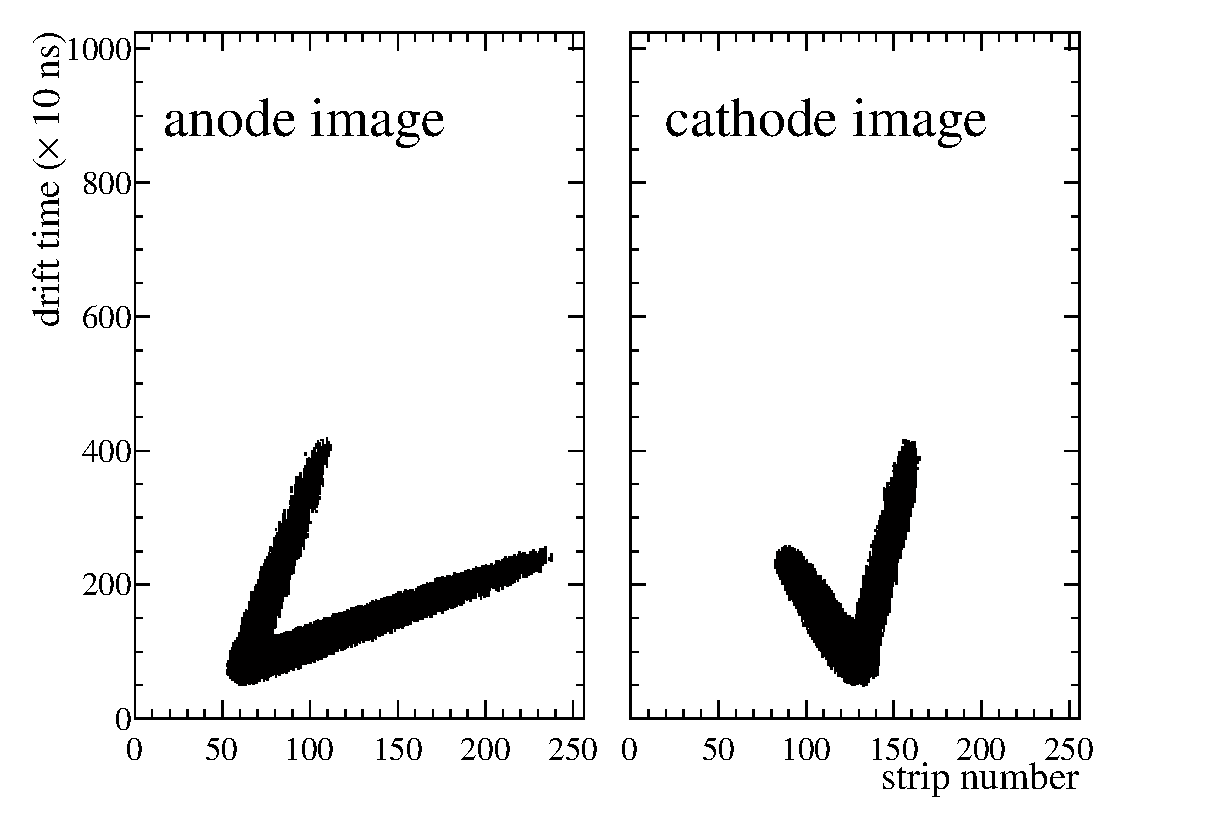
\includegraphics[clip, width=0.8\columnwidth]{10024_25.eps}
  \caption{2本しかトラックを確認できないイベントの画像 (\isoButaneHydro の場合).}
  \label{fig::not_three_alpha_ic4h10_h2}
\end{figure}
\begin{figure}
  \centering
  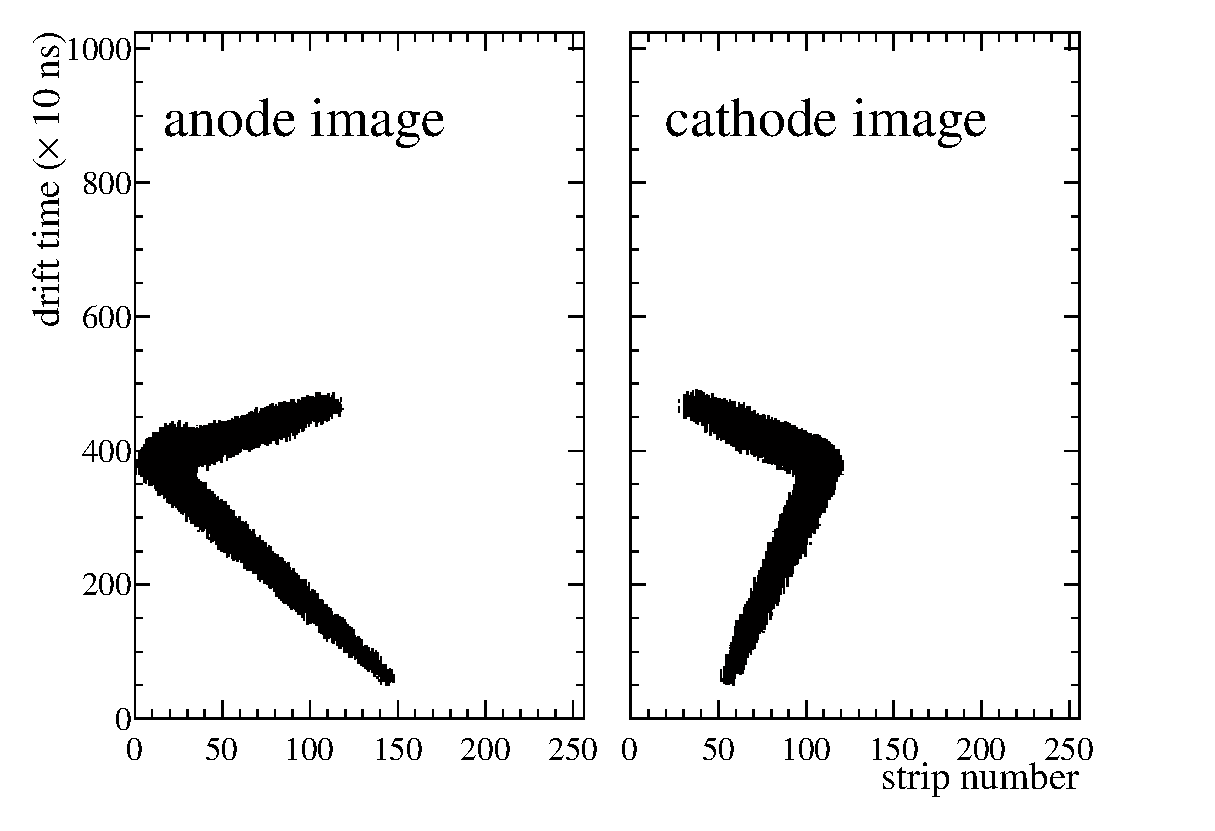
\includegraphics[clip, width=0.8\columnwidth]{10023_32.eps}
  \caption{2本しかトラックを確認できないイベントの画像 (\isoButaneHerium の場合).}
  \label{fig::not_three_alpha_ic4h10_he}
\end{figure}

\end{document}
